\documentclass[
  12pt,
  a4paper,
  parskip,
  openany
]{scrbook}

\usepackage{scrhack}
\usepackage[utf8]{inputenc}
\usepackage[english]{babel}

\usepackage[hidelinks, pdfpagelabels, pdfusetitle]{hyperref}
\hypersetup{hypertexnames=false}
\usepackage{enumitem}
\usepackage{suffix}
\usepackage{lipsum}
\usepackage{tabularx}
\usepackage{graphicx}
\usepackage[title,titletoc,header,toc,page]{appendix}
\renewcommand{\appendixname}{Appendix}

% Layout refinements
% Also fixes overfull hbox due to texttt
\usepackage{microtype}

% Abbreviations
\usepackage{glossaries-extra}
\setabbreviationstyle{long-short}
\setabbreviationstyle[acronym]{long-short}
\makeglossaries
% Reference abbreviation entry, do not remove in PR
\newabbreviation{foobar}{FOOBAR}{fully operational organization building acronym references}


\newacronym{sql}{SQL}{Structured Query Language}
\newacronym{cql}{CQL}{Cassandra Query Language}
\newglossaryentry{nosql}{
  name={NoSQL},
  description={
    \textit{No SQL} or \textit{Not only SQL}.
    NoSQL is a loosely defined term, grouping different
    databases which either do not only support data
    accesses via the Structured Query Language (SQL),
    or do not support it at all.
  },
}

\newacronym{crud}{CRUD}{Create, Read, Update, Delete}
\newacronym{api}{API}{Application Programming Interface}
\newacronym{mdm}{MDM}{Master Data Management}
\newacronym{it}{IT}{Information Technology}
\newacronym{orm}{ORM}{object-relational mapping}
\newacronym{ogm}{OGM}{object-graph mapping}
\newacronym{rdbms}{RDBMS}{relational database management system}
\newacronym{iam}{IAM}{identity and access management}
\newacronym{oltp}{OLTP}{online transaction processing}
\newacronym{acid}{ACID}{Atomicity, Consistency, Isolation, Durability}

\newglossaryentry{cern}{
  name={CERN},
  description={
    CERN, the European Organization for Nuclear Research, is one of the world's
    largest and most respected centres for scientific research.
  },
}
\newglossaryentry{atlas}{
  name={ATLAS},
  description={
   ATLAS (A Toroidal LHC ApparatuS) is one of the seven particle detector
   experiments at the Large Hadron Collider (LHC), a particle accelerator at CERN.
   It generates 1 petabyte of raw data per second, even after filtering it
   still requires over 100 megabytes of disk space per second – at least a
   petabyte each year \autocite{fermi2004giant}.
  },
}


% Listings and drawings (needs to be loaded before csquotes)
\usepackage{minted}
\usepackage{tikz}
\usetikzlibrary{intersections,arrows.meta}


% Citation packages and options
\usepackage{csquotes}
\usepackage[
  backend=biber,
  style=apa,
]{biblatex}
\addbibresource{bibliography.bib}

\DeclareLanguageMapping{english}{english-apa}


% Correct listing references
\providecommand*{\listingautorefname}{Listing}

% ===== INDIVIDUAL AUTHORS PER CHAPTER =====
% Source: https://tex.stackexchange.com/a/156865
\newcommand\chapterauthor[1]{\authortoc{#1}\printchapterauthor{#1}}
\WithSuffix\newcommand\chapterauthor*[1]{\printchapterauthor{#1}}

\makeatletter
\newcommand{\printchapterauthor}[1]{%
  {\parindent0pt\vspace*{-25pt}%
  \linespread{1.1}\large#1%
  \par\nobreak\vspace*{35pt}}
  \@afterheading%
}
\newcommand{\authortoc}[1]{%
  \addtocontents{toc}{\vskip-10pt}%
  \addtocontents{toc}{%
    \protect\contentsline{chapter}%
    {\hskip1.3em\mdseries\protect\scriptsize#1}{}{}}
  \addtocontents{toc}{\vskip5pt}%
}
\makeatother
% ==========================================


\title{NoSQL Databases}
\author{Daniel Rutz and Leon Schürmann (Eds.)}
\date{\today}

\begin{document}

\maketitle
\tableofcontents


\printglossaries


\chapter{Test}
\chapterauthor{Foo, Bar}

First use: \gls{foobar}.
Second use: \gls{foobar}.


\chapter{Key Value Introduction}
\chapterauthor{Vanessa Jörns, Tobias Schiffmann and Victor Veal}
Key-value databases or key-value stores are a classification of NoSQL databases. 
The idea of key-value stores is to collect a key  for every data set. Each set that is stored in the database can be accessed by the key. Therefore the key needs to be distinct, whether in a namespace or in the whole system. The database system has no pattern for the values which is why it is not  necessary to know about the type of the values that are stored. This feature enables easy storage of any kind of data like serialized structures, XML, text data, files...  \parencite{keyValueIntro}.


However, there are also disadvantages of this database management type. In terms of operational actions like querying through the data, as one would do in relational database management systems, key-value databases only provide simple operations like get, put and delete. As a result of this constraint, data querying must be handled at the application level. 

Another difference to relational databases are the use cases. 
 For simple applications, which only require a system that is able to store and manage data (e.g. update entries, join tables), is capable of representing real-world entities and describes relationships, relational databases should be used. Key-value databases should rather be chosen if the application or the system requires a good performance since key-value solutions are faster than relational database systems \parencite{keyValueUsecase}.
 
For instance, an online application that is only responsible to enable quick access to a profile, does not need to interact with entries of the profile itself. It should rather guarantee that the user of the application can easily find the profile by providing the corresponding key. To enable a quick access of the profile, it would be enough to only search for the unique ID of the profile instead of querying across several attributes of the data set.

Nevertheless, not all key-value solutions are similar designed. There are a lot of different systems today. In the following chapters some database management systems will be introduced. The focus will be on providing the reader a quick overview about the different systems, how they distinguish from each other and how to use them.

The first system that will be explained is Hazelcast which gives an overview of the the basic characteristics including a cheat sheet with needed commands. The next section talks about Redis and the basic features as well as in-memory computing. Last but not least the Key Value chapter is finished with a section about Riak. 


% eventuell Bild
% [1] https://en.wikipedia.org/wiki/Key-value_database#/media/File:KeyValue.PNG

\chapter{Hazelcast}
\chapterauthor{Vanessa Jörns, Tobias Schiffmann and Victor Veal}

\section{Hazelcast Introduction}

Hazelcast is a company that is developing an in-memory computing platform consisting of Hazelcast IMDG, Hazelcast Jet and Hazelcast Cloud. “Hazelcast Jet is an embeddable, distributed computing platform for fast processing of big data sets”. It is built on the foundation of Hazelcast IMDG on which this chapter focuses \parencite{hazelcast}.

An in-memory data grid (IMDG) is a rather new concept where data is stored in the main memories of a computing cluster. One of the main aspects is the ability to automatically scale and rebalance the cluster when decreasing or increasing in size. Here the data is partitioned equally across the cluster nodes. IMDGs are usually used for implementing distributed and scalable applications since they provide distributed versions of the basic data structures \parencite{tasci2015}. Hazelcast IMDG is open source and implemented in Java. However, there are also existing API’s for C/C++, .NET, REST, Python, Go and Node.js.

As Hazelcast is designed to be lightweight and easy to use, it can be downloaded as a compact library (JAR) and can be used by simply adding this JAR file to the classpath. With Java as the only dependency there is no need to install any software \parencite{hazelcastmanual}.

Firstly, the features of Hazelcast are specified and distinguished from other key-value solutions. The next section talks about the CAP theorem and how it applies to Hazelcast. After that a short manual for implementing Hazelcast for own applications is provided. This inlcudes a basic set up as well as a configuration. For reference a cheat sheet with the most important commands is included. In the end, the whole chapter about Hazelcast is concluded and the advantages and disadvantages are analyzed. 
\section{Specification}
Hazelcast consists of many same or similar features like other key value databases and IMDGs. However, there are some major features which describe Hazelcast’s distinctive strengths.
The first and one of the main characteristics is that Hazelcast completely computes in-memory rather than storage based.  This makes Hazelcast extremely fast but also volatile.

Another major feature is that Hazelcast relies on clustering with the approach of a “masterless nature” of the nodes. This means that each node in the cluster has the exact same functionality and operates in a peer-to-peer manner \parencite{johns2015}. So unlikely other NoSQL databases, there is no master and slave hence there is no single point of failure. All nodes are responsible for the same proportion of processing and storing \parencite{hazelcastmanual}. The oldest node of the cluster automatically becomes the “de facto leader” and manages the distribution of the data for joining nodes. Since the data is redistributed for every joining or exiting node, the cluster rebalances automatically and thus makes Hazelcast simple to set up and configure.

As Hazelcast consists of the basic features of an in-memory data grid, the data and therefore the load is equally spread across the cluster. Here each node is the owner and holds a number of partitions of the overall data.
Therefore, saturation of a cluster can simply be overcome by adding more nodes to the cluster. The cluster is then rebalanced and the load for each node decreases. This means scaling is easy and fast which makes Hazelcast suitable for handling big amounts of data.
Nevertheless, since Hazelcast persists data entirely in-memory, it has the main drawback that data will be lost with a node shutting down. To prevent the overall cluster of losing the data a failing node has held, Hazelcast distributes backups of each data partition among multiple other members. This means in case of a node shut down, another node will have a backup of the data and the cluster can be rebalanced without suffering any data loss and downtime \parencite{johns2015}.
\begin{figure}[H]
    \centering
    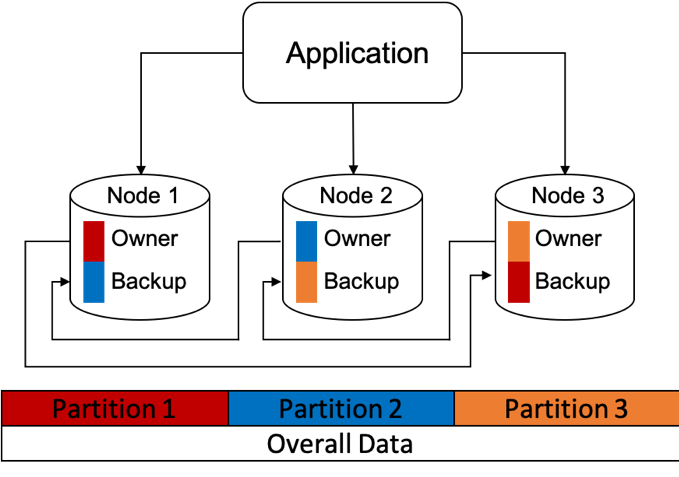
\includegraphics[scale=0.6]{img/hazelcast-nodes.png}
    \caption{Hazelcast Nodes \parencite{johns2015}}
\end{figure}
This illustration shows the cluster structure as described above. It explains how the data is partitioned in equal parts and spread across the cluster as well as the replication of the data for backup. This is just a simplified version of the structure with only three nodes. In practice each node would be responsible for multiple subsets of the data and not just one data partition. So, for instance in order to get the data of Partition 1, the application has to communicate with Node 1. The distribution of the data is dynamic and which node is responsible for which subset of data usually changes over time. Hence, the allocation is an internal operational detail and the application as well as the user usually does not need to know it.
Moreover, Hazelcast supports various distributed collectors, features and processors. Besides storing the data in-memory distributed on many nodes, it is possible to load data from diverse sources into varying structures, communicate across the cluster by sending messages and to use the stored data for analytical processing \parencite{johns2015}.


\section{Hazelcast and the CAP theorem}
As Hazelcast enables data storage for distributed systems, it may be interesting how the CAP theorem applies to it. According to the chapters before, Hazelcast offers a storage mechanism that distributes data across several nodes. Therefore the first aspect out of the CAP theorem is network partitioning. According to the article \textit{Jepsen Analysis on Hazelcast 3.8.3} \parencite{hazelcastCP}, Hazelcast is a PA system which means that it favours availability over consistency. Due to the fact that data is partitioned, the problem of keeping the data consistent over the whole system occurs. For example, if the user inserts a new entry to a cluster, the whole systems needs to update this info so that the same information can be provided from all nodes. This problem of having several nodes storing inconsistent data is called split brain in an In-Memory Data Grid system.

Hazelcast offers a method that should avoid split brain. In the so called "Split Brain Protection" a minimum number of nodes is set on which write or read operations are prevented. If a split brain happens, any sub-clusters that have a lower number of nodes than the minimum number are prevented from accepting write operations. Nevertheless, this method only reduces the time of inconsistency. Therefore it does not completely avoid the inconsistent state of the system \parencite{hazelcastCP}.

Recently, the Hazelcast company has announced the ability to provide a solution that supports both PA (availability over consistency) and PC (constistency over availability). This feature should allow the user to adapt more flexibly to the requirements of the application. So far, there are too less resources that can describe this new feature of Hazelcast which is why this paper is currently not able to report about it \parencite{hazelcastCAP}.

\section{Implementation}
\subsection*{Getting Started}
As already mentioned Hazelcast is designed to be easy to use and therefore only require a few steps to set it up running.
First of all, the Hazelcast package has to be downloaded, for example from the official website \parencite{hazelcast:hazelcastDownload}. The package is offered in a compressed data format and has to be extracted afterwards.

Hazelcast does not need any software installations. It is written in Java and therefore the platform to run Hazelcast on needs to be able to execute Java code. To do so a Java Development Kit has to be ready to use which can be gathered from the Oracle website. After ensuring Java code to run, Hazelcast is ready to be used.

The console application is an easy way to get in touch with Hazelcast and experience the software. It can be started by executing the \texttt{console} scripts in the \texttt{demo/} directory from a terminal. Hazelcast creates a new member which will either create a new cluster or will join a cluster if there already exists one. The cluster can than be filled by typing the commands as the following example shows.
\begin{flushleft}
\begin{figure}[h]
    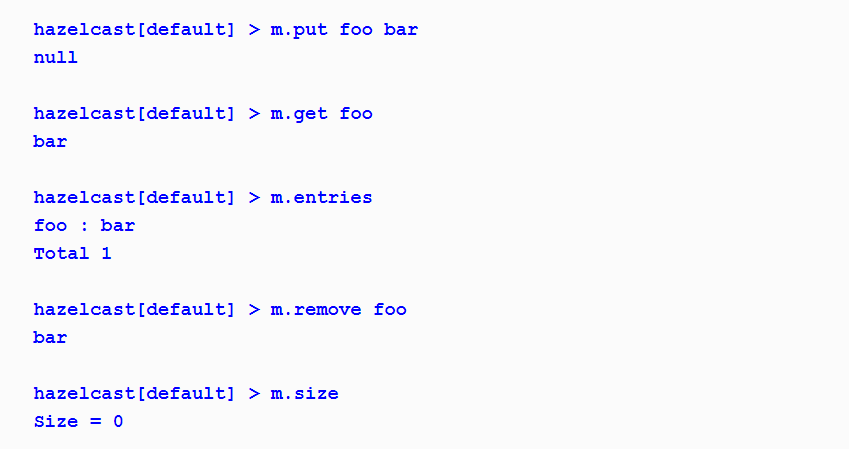
\includegraphics{img/hazelcastPut.PNG} 
    \caption{Hazelcast Basic Commands \parencite{johns2015}}
\end{figure}
\end{flushleft}
When executing the scripts in another window, Hazelcast shows how the new member joins the cluster and displays the two members and there addresses after a short period of time.

\begin{flushleft}
\begin{figure}[h]
    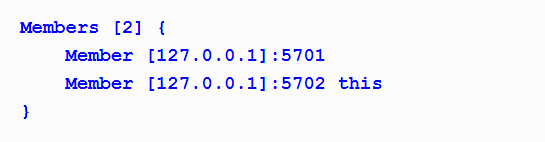
\includegraphics{img/hazelcastMembers.PNG}
    \caption{Example Member List \parencite{johns2015}}
\end{figure}
\end{flushleft}
Now the data is spread across the members. They both own a particular partition of the data and store the other part as backup.

When closing one terminal to test Hazelcast's reaction to a cluster node failure, the remaining member tries to reestablish the connection to the closed one, but without success. The terminal will than display the process of repartitioning the cluster and prints a statement when it finishes.
\subsection*{Members and Clients}
Besides the console application Hazelcast also provides the opportunity to include the Hazelcast package in your code. For Java there is a package for members and one for clients provided. Other programming languages only have clients to work with. The difference between clients and members is that clients do not hold data. They connect to Hazelcast cluster members and access the data on that way for read and write operations \parencite{hazelcastmanual}. If Hazelcast has to be set up for an application in C++ for example, the scripts in the \texttt{demo/} directory can be used to start a cluster member without needing to create a java application. The C++ application than has to include the Hazelcast package and can access or create the data via the member.
\subsection*{Configuration}
Hazelcast offers an XML file to adjust certain configurations in the \texttt{bin/} directory.
It is possible to change the amount of backups and also the types of backups. There are normal backups which are synchronized and therefore lock the data in case it is manipulated. All other nodes have to wait until the data is changed in all backups and the changes are confirmed by the nodes which hold the backups. Additionally, there are asynchronous backups. They do not lock any data and therefore bring a performance increase because the nodes do not have to wait for them to confirm the changes. On the other hand, it brings the risk of inconsistent data. Nodes could access data which are no longer valid because the changes were not made on all backups after a manipulation took place.

In general, increasing the number of backups will increase the read performance because the data can be read on different nodes in parallel. The costs for this advantage are either bad write performance in case of normal backups or inconsistency in case of asynchronous backups.

Furthermore Hazelcast provides configurations about how big a particular data structure can grow and how to act when there is no more space left. 
\begin{flushleft}
\begin{figure}[h]
    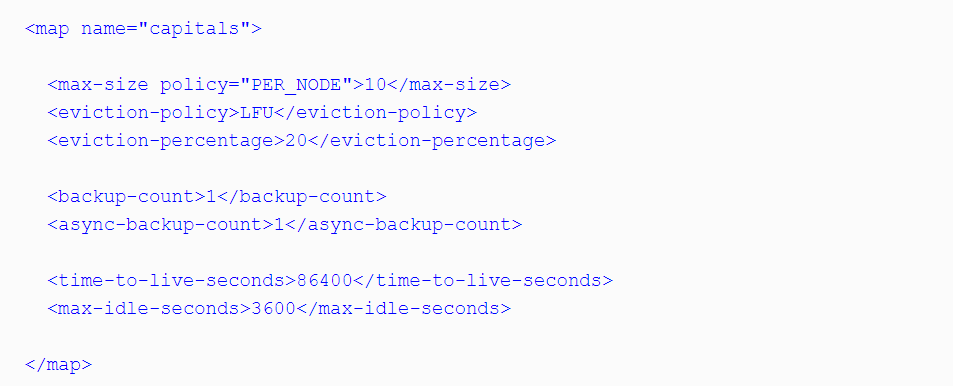
\includegraphics{img/hazelcastXML.PNG}
    \caption{Hazelcast Configuration \parencite{johns2015}}
\end{figure}
\end{flushleft}
In this example the map called \textit{"capitals"} has a maximum size of 10 items per node. When reaching this maximum, 20 percent of the data will be freed according to the principle of Least Frequently Used (LFU). One synchronous and one asynchronous backup will be created and the time to live for data sets is set. This means that data will be deleted after this amount of seconds goes by. In contrast to this, setting the maximum idle time will only delete a data set when it is not accessed after a certain amount of seconds.
\citeauthor{johns2015} and the Hazelcast websites provide more information about configuration and go more in detail.

\section{Cheat Sheet}
\subsection*{General commands}
\begin{tabular}{|p{0.3\textwidth}|p{0.7\textwidth}|}
    \hline
    \texttt{echo true|false} & turns on/off echo of commands (default false)\\\hline
    \texttt{silent true|false} & turns on/off silent of command output (default false)\\\hline
    \texttt{\# <number> <command>}& repeats \texttt{<number>} time \texttt{<command>}, replace \$i in \texttt{<command>} with current iteration (0...\texttt{<number-1>)}\\\hline
    \texttt{\& <number> <command>}& forks \texttt{<number>} threads to execute \texttt{<command>}, replace \$t in \texttt{<command>} with current thread number ((0...\texttt{<number-1>)})\\\hline
    \texttt{jvm} & displays info about the runtime\\\hline
    \texttt{who} & displays info about the cluster\\\hline
    \texttt{whoami} & displays info about this cluster member\\\hline
    \texttt{ns} \texttt{<string>} & switch the namespace for using the distributed queue/map/set/list \texttt{<string>} \newline (default value = "\texttt{default}")\\\hline
    \texttt{@ <file>} & executes the given \texttt{file} script. Use '//' for comments in the script\\\hline
\end{tabular}
\subsection*{Queue commands}
\begin{tabular}{|p{0.3\textwidth}|p{0.7\textwidth}|}
    \hline
    \texttt{q.offer <string>} & adds a string object to the queue\\\hline
    \texttt{q.poll} & takes an object from the queue\\\hline
    \texttt{q.offermany <number> [<size>]} & adds indicated number of string objects to the queue ('\texttt{obj<i>}' or \texttt{byte[<size>]})\\\hline
    \texttt{q.pollmany <number>} & takes indicated number of objects from the queue\\\hline
    \texttt{q.iterator [remove]} & iterates/displays the queue, remove if specified\\\hline
    \texttt{q.size} & adds a string object to the queue\\\hline
    \texttt{q.clear} & clears the queue\\\hline
\end{tabular}
\subsection*{Set commands}
\begin{tabular}{|p{0.3\textwidth}|p{0.7\textwidth}|}
    \hline
    \texttt{s.add <string>} & adds a string object to the set\\\hline
    \texttt{s.remove <string>} & removes the string object from the set\\\hline
    \texttt{s.addmany <number>} & adds indicated number of string objects to the set ('\texttt{obj<i>}')\\\hline
    \texttt{s.removemany <number>} & takes indicated number of objects from the set\\\hline
    \texttt{s.iterator [remove] } & iterates/displays the set, removes if specified\\\hline
    \texttt{s.size} & size of the set\\\hline
    \texttt{s.clear} & clears the set\\\hline
\end{tabular}
\subsection*{List commands}
\begin{tabular}{|p{0.3\textwidth}|p{0.7\textwidth}|}
    \hline
    \texttt{l.add <string>} & adds string to the list\\\hline
    \texttt{l.add <index> <string>} & adds string at a certain index\\\hline
    \texttt{l.contains <string>} & checks if list contains \texttt{<string>}\\\hline
    \texttt{l.remove <string>} & removes \texttt{<string>} from list\\\hline
    \texttt{l.remove <index>} & removes element at \texttt{<index>} from list\\\hline
    \texttt{l.set <index> <string>} & replaces value at \texttt{<index>} with \texttt{<string>}\\\hline
    \texttt{l.iterator [remove]} & iterates/displays the list\\\hline
    \texttt{l.size} & size of list\\\hline
    \texttt{l.clear} & clears list\\\hline
\end{tabular}
\subsection*{Map commands}
\begin{tabular}{|p{0.3\textwidth}|p{0.7\textwidth}|}
    \hline
    \texttt{m.put <key> <value>} & puts an entry to the map\\\hline
    \texttt{m.remove <key>} & removes the entry of given key from the map\\\hline
    \texttt{m.get <key>} & returns the value of given key from the map\\\hline
    \texttt{m.putmany <number> [<size>] [<index>]} & puts indicated number of entries to the map ('\texttt{key<i>}':\texttt{byte[<size>]}, \texttt{<index>+(0..<number>})\\\hline
    \texttt{m.removemany <number> [<index>]} & removes indicated number of entries from the map ('\texttt{key<i>}', \texttt{<index>+(0..<number>})\\\hline
    \texttt{m.keys} & iterates/displays the keys of the map\\\hline
    \texttt{m.values} & iterates/displays the values of the map\\\hline
    \texttt{m.entries} & iterates/displays the entries of the map\\\hline
    \texttt{m.iterator [remove]} & iterates/displays the keys of the map, remove if specified\\\hline
    \texttt{m.size} & size of the map\\\hline
    \texttt{m.localSize} & local size of the map\\\hline
    \texttt{m.clear} & clears the map\\\hline
    \texttt{m.destroy} & destroys the map\\\hline
    \texttt{m.lock <key>} & locks the key\\\hline
    \texttt{m.trylock <key>} & tries to lock the key and returns immediately\\\hline
    \texttt{m.trylock <key> <time>} & tries to lock the key within given seconds\\\hline
    \texttt{m.unlock <key>} & unlocks the key\\\hline
    \texttt{m.stats} & shows the local stats of the map\\\hline
\end{tabular}
\subsection*{MultiMap commands}
\begin{tabular}{|p{0.3\textwidth}|p{0.7\textwidth}|}
    \hline
    \texttt{mm.put <key> <value>} & puts an entry to the multimap\\\hline
    \texttt{mm.get <key>} & returns the value of given key from the multimap\\\hline
    \texttt{mm.size} & size of the multimap\\\hline
    \texttt{mm.clear} & clears the multimap\\\hline
    \texttt{mm.destroy} & destroys the multimap\\\hline
    \texttt{mm.iterator [remove]} & iterates the keys of the multimap, remove if specified\\\hline
    \texttt{mm.keys} & iterates/displays the keys of the multimap\\\hline
    \texttt{mm.values} & iterates/displays the values of the multimap\\\hline
    \texttt{mm.entries} & iterates/displays the entries of the multimap\\\hline
    \texttt{mm.lock <key>} & locks the key\\\hline
    \texttt{mm.trylock <key>} & tries to lock the key and returns immediately\\\hline
    \texttt{mm.trylock <key> <time>} & tries to lock the key within given seconds\\\hline
    \texttt{mm.unlock <key>} & unlocks the key\\\hline
    \texttt{mm.stats} & shows the local stats of the map\\\hline    
\end{tabular}

\section{Conclusion}

Hazelcast is categorized as a key-value NoSQL solution, but since it is an in-memory data grid there are some main features that should be emphasized which set Hazelcast apart from the ordinary key-value databases.
First of all, one of the key characteristics is its simplicity. As mentioned above, Hazelcast’s only dependency is Java and therefore it can be used by simply downloading the JAR file and including it in the classpath.
Furthermore, the cluster is structured as a peer-to-peer network, meaning there is no master-slave relation which is usually common for NoSQL databases. Each node is responsible for the same amount of data.

Another characteristic is the speed of Hazelcast since it relies on in-memory computing \parencite{hazelcastmanual}. Knowingly in-memory computing also comes with two main downsides: volatility and scalability. Hazelcast, however addresses these issues.
Volatility is solved by keeping the data of the nodes redundant. This means that Hazelcast stores the data of each node on multiple members. So, if one member fails, there is a backup and the whole cluster can be rebalanced and there is no overall loss of the data.
Scalability is achieved by just adding more nodes to the cluster, the data is then automatically rebalanced and the work load for each member decreases.

These main features of Hazelcast also directly conclude some major advantages. To summarize the already mentioned ones, Hazelcast is very easy and fast to install and it is designed to provide fast computing. Additionally, since there is no master-slave concept, there is also no single point of failure. It is easy to scale either up or down and redundant data storage protects from unexpected data loss \parencite{hazelcastnosql}.
Furthermore, in contrast to ordinary key-value databases, Hazelcast is designed for a distributed environment and therefore it is possible to provide an unlimited number of maps and caches per cluster. Another advantage is that Hazelcast can be implemented using multiple threads and thus benefits from all available CPU cores \parencite{hazelcastredis}.

Nevertheless, Hazelcast relying entirely on in-memory processing still comes with the drawback that this kind of storage is temporary. So, in case there is an overall system shut down the data is lost since the backups are stored in the same cluster. In addition, RAM is usually expensive which should be kept in mind when considering scalability.

Regarding the CAP theorem, as discussed above, Hazelcast can be either implemented as an PA or PC system. When using Hazelcast as a PA system, it is neglecting consistency. Meaning the system is not fully consistent all the time. On the other hand, in case of a PC system, it fails to provide continuous availability.
Furthermore, as a PC system the speed of the data grid system relies on the slowest node. If backups are kept synchronously, data is locked until the consistent state is achieved again \parencite{johns2015}. The other nodes will have to wait until this particular block of data is unlocked again.


Hazelcast provides several and detailed manuals online as well as understandable tutorials which makes it easy to adapt Hazelcast for own applications. However, scientific research and benchmarking is very limited.
\chapter{Key-value databases}
\section{Redis}
\chapterauthor{Laura Khaze, Leon Sch\"urmann}

Redis is a key-value data store. It was invented by Salvatore Sanfilippo in
April 2009 and is released under the \gls{bsd} 3-clause (\textit{new} /
\textit{revised}) license. Therefore, it is a free and open source software
product. Redis -- originally an acronym for \textit{remote dictionary server} --
is primarily used as a database, caching-solution or a publish/subscribe message
broker.

Redis stands out in the field of key-value data stores because of its simplicity
and speed. A part of the high performance can be attributed to the use of
in-memory data structures, while the use of C -- a low-level systems programming
language -- provides some advantages as well. Because of its unique properties,
Redis is very popular. According to \texttt{db-engines.com}, it is currently on
rank seven of the most popular databases, and on rank one of all measured
key-value data stores \parencite{dbenginesRanking}.

The goal of this section is to show the primary characteristics and available
data types of Redis. Clustered Redis setups will be evaluated in the context of
the \gls{cap}. Finally, typical usage scenarios for this software will be
evaluated, and the most important facts are reiterated in the conclusion.

\subsection{Primary characteristics}
Redis has a few distinctive characteristics that make it unique in the set of
\gls{nosql} databases covered by this book. This section will evaluate these
characteristics in regards to the overall influence on the software.

\subsubsection*{In memory}
Redis is designed to run completely \textit{in-memory}
\parencite{redis:introduction}.  Traditional databases rely on their data being
stored on a hierarchical file system, typically on top of a mass storage medium
like \glspl{hdd} or \glspl{ssd}. While these media often come in
much larger sizes than \gls{ram} modules, and have a significantly less cost
per gigabyte, storing data on them has a few drawbacks.
For instance with \glspl{hdd}, accessing data at a specific position on the
disk requires waiting for a data seek operation to complete -- essentially
letting the physical platter spin to the sector where data is stored and moving
the read/write head into position. This makes random read and write operations
slow. Even with flash-based storage like \glspl{ssd}, where seeking data is not
an issue, there are many layers of abstraction between the virtual file system
and the physical data storage. Accessing a file on file systems typically
involves performing a so-called \textit{context switch} into the operating
system kernel, accessing a hardware controller, serializing data over a wire
according to standards like \acrshort{sata}, and the disk controller finally
accessing the data. All of these operations take a considerable amount of time.
\parencite{edgar}
However, when an application accesses its own main memory region in the system's
\gls{ram}, these operations get processed natively in the \gls{cpu} and
\gls{iommu} hardware, without involvement of the operating system kernel or any
peripherals.

In summary, storing data in \gls{ram} has advantages to system load, seek times,
response times and available bandwidth. However, at the time of writing,
\gls{ram} is significantly more expensive than traditional storage media. The
cost per gigabyte ratio could be higher then 238x (when comparing recent prices
of a $512GB$ \acrshort{ddr4} \acrshort{ecc} memory stick with a $4TB$ $7200rpm$
enterprise \gls{hdd}).

Because \gls{ram} is a form of volatile memory, after a power loss or system
reset, the data is cleared. To prevent data loss with Redis, two types of
persistence modes can be used \parencite{redis:persistence}:
\begin{itemize}
    \item \textbf{\texttt{RDB} files}:\\
	Redis can dump its entire data set into a binary \texttt{RDB} file that
        is sufficient to restore a full and consistent snapshot of a Redis instance.
        However, creating this dump takes time and memory -- Redis forks its primary
        process and therefore duplicates the entire in-memory data set. Copy-on-write
        techniques can reduce system load with this process. It is unfeasible to use
        this method for continuously storing the database's state.
        \parencite{redis:persistence}

    \item \textbf{\texttt{AOF} files}:\\
	Redis logs all of its transactions into an \texttt{AOF} file which can
        then be used to reconstruct a full snapshot of a Redis instance. This file has
        the advantage of being append-only, reducing random accesses and seek times. In
        addition to that, new transactions can be constantly written to this file
        without interrupting the primary Redis thread. However, as new transactions can
        make old ones irrelevant, these files are often not as compact as \texttt{RDB}
        database dumps. Therefore, they can be compacted to contain only required
        transactions to rebuild the current database state. \parencite{redis:persistence}
\end{itemize}

\subsubsection*{\acrshort{resp}: \acrlong{resp}}
To communicate with a Redis instance, a client has to use the \gls{resp}. The
primary goals of this protocol are to be simple to implement, fast to parse and
to be human readable. While it only relies on a bidirectional communication
channel with some guarantees regarding safety and packet order, it is currently
only implemented on top of \gls{tcp} or UNIX sockets. \parencite{redis:protocol}

\gls{resp} is designed to adhere to a request-response pattern. Both the
requests to the server instance, as well as the responses have a well-defined
human readable format. Different parts of the protocol are always terminated
with a carriage-return and new-line character (\texttt{CR LF} or
\texttt{\char`\\ r\char`\\ n}). \parencite{redis:protocol}

Each request is an array of a Redis command and additional string arguments. The
length of the array, as well as the size of all strings is sent as a prefix to
the respective element. This has the advantage of being both simple to construct,
and Redis being able to allocate a fixed size chunk of memory for each element.
Therefore, once the data is received, no post-processing is required.
\parencite{redis:protocol}

The response for a request always starts with an \acrshort{ascii}-byte
indicating the response data-type. For instance, this could be "\texttt{-}" for
a string error, or "\texttt{:}" for a string-encoded integer that is guaranteed
to be a valid $64$ bit signed integer value. Following this byte, the payload is
encoded as a (depending on the type \textit{binary safe}) string.
\parencite{redis:protocol}

Overall, the Redis protocol achieves its goals of speed, simplicity and human
readability. Its properties make it easy to develop libraries for communication
with Redis.

\subsection{Data Types} \label{redis:dataTypes}
Redis is not only a key-value data store but rather a data structures server. In a
classical key-value data store a string value is accessed via a string key while
Redis supports several other data structures (hashes, sorted sets, etc.). The
basic data structures as well as some extraordinary ones will briefly be
described in this section. \parencite{redis:dataTypesIntroduction}

\subsubsection*{Strings}
Strings are the most basic data type used in a Redis data store on which all
complex data structures are built. Strings are binary safe, which means it is
possible to save any kind of data (max 512MB per key), like a \gls{jpeg}
image or a serialized Ruby object, as well as simple text.

Moreover, it is possible to use strings as atomic counters using commands in the
\texttt{INCR} familiy (\texttt{INCR}, \texttt{INCRBY}, etc.). Since it is not
possible to declare an integer in Redis, strings are used for those purposes.
Furthermore, it is possible to use strings as random access vectors due to
commands like \texttt{GETRANGE}, \texttt{SETRANGE} or \texttt{GETBIT}.
\parencite{redis:dataTypesIntroduction, redis:commands, redis:dataTypes}

\subsubsection*{Lists}
Redis lists are a collection of strings sorted by insertion order with a maximum
length of $2^{32}-1$ strings. Among other operations, it is possible to insert
and delete elements within a list (either from the head or tail), as well as
getting a subset of a list. A list is created when a push operation is
performed on an empty key and conversely a list is deleted (key clearance) if
the list is emptied by an operation.

Due to the combination of some operations, it is possible to create a customized
list for specific use cases. For instance, it is possible to use \texttt{LPUSH}
and \texttt{LTRIM} to create a list with a defined length which will never
exceed a certain number of elements.  Moreover lists can be used to model a
timeline in a social network like Instagram or Facebook. In this example it
would be possible to add new elements in the time line (\texttt{LPUSH}) and
receive only the most recent events (\texttt{LRANGE}).
\parencite{redis:dataTypesIntroduction, redis:commands, redis:dataTypes}

\subsubsection*{Sets}
Unlike lists, sets are an \textit{unordered} collection of strings with a
maximum number of $2^{32}-1$ elements.
Elements within a set are called members. Members can be added, removed and
returned from a set (\texttt{SADD}, \texttt{SREM}, \texttt{SPOP}). If a string
is already contained within the set, it is not possible to add it again. In this
case, Redis will simply not add the member, without indication of an error.
Thus, it is not necessary for an application to use \texttt{SISMEMBER} before
calling the \texttt{SADD} operation on a set. Moreover it is possible to display
all members of a set and check whether a specific member is contained within a
set (\texttt{SMEMBER}, \texttt{SISMEMBER}).

Due to the characteristics of the \texttt{SADD} function, sets can be used to
track unique things like students ids lending a specific book in the library.
\parencite{redis:dataTypesIntroduction, redis:commands, redis:dataTypes}

\subsubsection*{Hashes}
Hashes are the most suitable data type to represent objects, since they are maps
between string fields and string values. Every hash can store up to
$2^{32}-1$ field value pairs.

It is possible to set fields and retrieve the value of fields, both either
individually or simultaneously (\texttt{HSET}, \texttt{HMSET}, \texttt{HGET},
\texttt{HMGET}). \parencite{redis:dataTypesIntroduction, redis:commands,
redis:dataTypes}

\subsubsection*{Sorted Sets}
Similar to sets, sorted sets are non repeating collections of strings ordered by
a non-unique score (smallest to greatest).  Members within a sorted set can be
added, removed and returned (\texttt{ZADD}, \texttt{ZPOPMIN}, \texttt{ZPOPMAX}).
Moreover it is possible to return members with a certain score or at a certain
position/index within the sorted set. Also, scores can be increased and thereby
updated.

Thus sorted sets can be used to keep track of any kind of ranking like a
competition. In this case, scores can be initially inserted and later updated using
\texttt{ZADD}.  Due to operations like \texttt{ZRANGE} or \texttt{ZRANK}, it is
possible to receive the top or bottom half of the ranking, or receive the rank
of a specific member. \parencite{redis:dataTypesIntroduction, redis:commands,
redis:dataTypes}

\subsection{Multi-node setups / Redis Cluster} \label{redis:multiNodeSetup}
Originally, Redis only supported single-node and non-clustered setups. In
combination with its mostly single-threaded architecture, this allowed it only
scale vertically.  However, with the introduction of both external clustering
mechanisms (where a so-called proxy would distribute and balance requests across
different Redis instances) and internal clustering support, Redis can now scale
horizontally as well. Because of the variety of clustering solutions, and focus
on Redis itself, external proxies are out of the scope of this evaluation.

The integrated clustering solution of Redis is called \textit{Redis Cluster}.
According to its documentation, \textit{"[it] is a distributed implementation
of Redis"} \parencite{redis:clusterSpecification} and has three primary goals:

\begin{itemize}
    \item \textbf{High performance and linear scalability} up to 1000 nodes
    \item \textbf{Write safety}
    \item \textbf{Availability}
\end{itemize}
However, by specification, these criteria do not have to be guaranteed at all
times -- altogether or even on their own. \parencite{redis:clusterSpecification}

Nodes in a Redis Cluster setup are connected over \gls{tcp} bus connections.
These connections (bus) are used to propagate information to all nodes in the
cluster. Client requests to nodes in the cluster are not forwarded to the
data-holding node. Instead, the client is redirected to the correct node by the
use of \texttt{MOVED} or \texttt{ASK} error return codes.
The data distribution is decided by the CRC-16 value of the string key. Each
unique CRC-16 value is called a keyslot. All keyslots have one master and
$n \geq 0$ slave nodes.
\parencite{redis:clusterSpecification}

\subsubsection*{Positioning in the CAP theorem}
In the following, different criteria of Redis Cluster regarding typical usage
guarantees in a distributed setup are evaluated:
\begin{description}
    \item \textbf{Consistency}:\\
        According to the official Redis website, \textit{"Redis is not able to
        guarantee strong consistency"} \parencite{redis:clusterTutorial}. This can be implied
        from a few scenarios.

        For instance, when a client writes a key to the respective master node
        for this keyslot, the operation is acknowledged instantly. The master then
        replicates this write to all slave-nodes for this keyslot. However, when these
        slave nodes are not reachable, the write is not fully synchronized across the
        network. In the case of a network partition, a slave that has not yet received
        this write operation may be promoted to become a master. The write is then lost,
        although it has been acknowledged. \parencite{redis:clusterTutorial}

	In another example, the network is partitioned into a master-majority and
        a master-minority partition. For a short amount of time, both partitions accept
        write operations which are also acknowledged. However, the minority-partition
        will eventually completely block any write operations. After the network is
        reunited, the previous writes to the minority-partition are simply discarded.
        Redis avoids merge operations, as these provide architectural challenges and
        might not work well on large data \parencite{redis:clusterSpecification}.
        \cite{redis:clusterTutorial}

    \item \textbf{Availability}:\\
	As already stated regarding the consistency of Redis Cluster, the
        minority-side of a network partition will refuse write-operations after a
        timeout. Therefore, Redis Cluster is not available.
        \parencite{redis:clusterSpecification}

	Even on the majority-side of the network, some write operations might be
        refused for a short amount of time. After an initial detection of a network
        partition and a timeout, slaves of missing keyslots get promoted to be master
        nodes. As soon as a master exists for all keyslots, the majority-partition is
        available again. \parencite{redis:clusterSpecification}
\end{description}

Depending on the kind of setup and test scenario Redis \textit{tends} to be
either AP or CP. Since this is only a small propensity, for systems or applications
requiring the characteristic AP or CP, a database designed for a clustering
solution should be used. This opinion is, in addition to the official documentation,
shared by \cite{redis:davis2015} and others.
Redis was initially designed as a single node solution with the primary focus on
performance.

\subsection{Typical use cases}
Redis can be used for a variety of different purposes and use cases. In the
following, three typical use cases are stated.

Redis can be used as a general purpose data store, especially if the data and
application requires simple data structures and high performance.  Nevertheless,
Redis is not suitable for every use case requiring a general purpose data store.
Since there are no complex data types, besides the ones mentioned in section
\ref{redis:dataTypes}, and it is not possible to model relations between
different data objects (as in a relational database), use cases with these
requirements can not be implemented using Redis. Moreover, the high memory usage
of Redis can either exceed the capacity of preexisting infrastructure, or
increase the cost of purchasing infrastructure drastically.

Due to these characteristics, Redis is often used to store volatile data, as a
caching mechanism or as a message broker. \parencite{redis:commands, redis:introduction}

\subsubsection{Caching}
Based on the characteristics of Redis, Redis is ideal for a caching mechanism.
Common \glspl{dbms} usually have high latencies and response times which could
make the user interface of an application feel sluggish.

\begin{figure}[h]
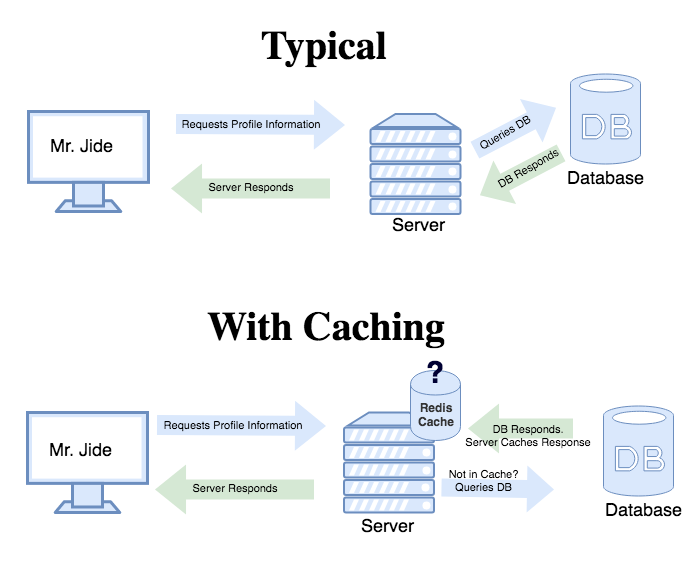
\includegraphics[width=12cm]{img/redis_caching.png}
\centering
\caption{Redis Caching Solution \parencite{redis:img:1}}
\label{fig:redisCaching}
\end{figure}

To solve this issue, a caching mechanism can be used. Already prepared and
computed data, which is used several times, is stored in the caching mechanism
with the result of less interaction between the user interface and the
\gls{dbms}.

In \textit{figure \ref{fig:redisCaching}}, the difference between server queries
to a database with and without Redis as a caching solution is pictured. The
second option (with a Redis cache) reduces the response time since only queries,
whose data is not already cached, are forwarded to the \gls{dbms}.

Redis-keys can be marked for deletion after a specified timeout (\texttt{TTL}),
and display the time that has elapsed since the key was last modified
(\texttt{OBJECT IDLETIME}). This enables automatic deletion of seldom used
data.  Thus Redis can be used as a caching solution for image previews, fetched
data from \acrshort{api}s, as well as session data. \parencite{redis:commands}

\subsubsection{Message broker functionalities}
Since Redis implements a publish-subscribe pattern, it is possible to use Redis
as a message broker.

A publish-subscribe pattern is a mechanism where subscribers can receive
information/messages from publishers. A typical publish-subscribe system
consists of several subscribers and several publishers, where one application can
be both subscriber and publisher. Publishers can provide information on specific
issues without any knowledge of possible subscribers. Each message is assigned
to a topic, which subscribers can subscribe to. In turn, these do not know if and
which publisher published on a specific topic. \parencite{redis:ibmPubSub}

Redis offers the typical publish-subscribe pattern features. Clients can
subscribe (\texttt{SUBSCRIBE}, \texttt{UNSUBSCRIBE}) to a topic as well as push
messages to a specific topic/channel (\texttt{PUBLISH}). The payload of the
message is a binary-safe string, which enables the clients to exchange any kind
of data.

This message broker functionality is especially useful for event notifications.
For instance the clients can be notified about changes within the data store.
Moreover, Redis' publish-subscribe implementation can be used to exchange
arbitrary data. However, because this is essentially a routed protocol, it is
less performant compared to peer to peer connections such as \gls{tcp} or UNIX
sockets. \parencite{redis:PubSub}

\subsection{Conclusion}
In this section, the key-value data store Redis was introduced by explaining the
main characteristics and some of Redis' data types. In addition to that, a
clustered Redis setup is analyzed in regards to characteristics from the CAP
theorem.  Finally, some of the most popular use cases were reiterated.

To summarize, Redis is much more than a traditional key-value data store.
Different data types, carefully chosen architectural decisions and a
speed-optimized implementation make it flexible and better suited for some
applications. For instance, Redis is an excellent data store for caching
purposes. While the publish- / subscribe feature does not necessarily have a
great influence on the storage features, it can be used in combination with
those to signal other Redis clients that some keys changed.

However, having a purely in-memory data store means that it is expensive to
operate with vast amounts of data. Also, data persistence is possible, but only
with a few disadvantages. Last but not least, Redis can be used in a clustered
setup. The internal clustering mechanisms (Redis Cluster) do not provide strong
guarantees regarding availability as well as consistency. This severely limits
its use-cases to applications, where both the correctness and presence of
distributed data is not a strict requirement.

\section{The Riak Key-Value Store}
\chapterauthor{Daniel Rutz, Paul Thore Flachbart}

\subsection{Introduction}
The Riak KV authors describe Riak KV as \enquote{a distributed \gls{nosql} database designed to deliver maximum data availability by distributing data across multiple servers. As long as your Riak KV client can reach one Riak server, it should be able to write data.} \parencite{RiakKV} Actually, this sentence already describes most of Riak's characteristics:
\begin{itemize}
	\item Riak has been developed with availability in mind. It constructs a distributed system of nodes without master node. Even though this system can't guarantee consistency, it makes sure that the database is available as long as one node is accessible.
	\item Riak is a \gls{nosql} database. Instead of using the \gls{sql} language, Riak provides an \gls{http} \parencite{RiakKVHTTP} and a Protocol Buffers \parencite{RiakKVProtoBuf} interface for \gls{crud} operations on key-value pairs.
\end{itemize}

There are two different databases besides Riak KV:
\begin{itemize}
	\item Riak TS has been developed for time series data. It is not scheme-free: You have to describe tables in a way similar to \gls{sql} \parencite{RiakTS}.
	\item Riak CS is a cloud storage solution. It has been developed to be compatible to the Amazon S3 \gls{api} \parencite{RiakCS}.
\end{itemize}

This chapter will deal with advantages and disadvantages of Riak KV. Furthermore, we will compare Riak KV to Redis and categorise it according to the CAP theorem. The other Riak\footnote{From now on, Riak KV will be referred to as Riak.} variants are not in the scope of this text.

\subsection{Characteristics of Riak}
Riak is a key-value store written in Erlang. According to \textcite{Kuznetsov2014}, it is inspired by the Amazon Dynamo whitepaper \parencite{DeCandia2007Dynamo}. Its main focus is distributivity: By using concepts such as consistent hashing and synchronisation using vector clocks, it does not need a master node to distribute data across multiple nodes.

Riak can be used in a {\itshape eventually consistent} or in a {\itshape strongly consistent} mode: When used with eventual consistency, an accessible Riak node will always answer to a request, but it cannot guarantee the response to be up-to-date. With strong consistency, Riak internally tries to solve the Byzantine Generals problem by achieving a distributed consensus between the nodes about the current value. If less than half the replications of a value are not available, however, Riak will not be able to return a response as the required quorum will not be reached. It should be noted that strong consistency is flagged as experimental; the Riak authors discourage its usage in production environments. \parencite{RiakStrongConsistency}

Riak splits its keyspace into so-called {\itshape buckets}. A key can be used multiple times as long as all the usages are in different keys. Access to a value must be done with bucket and key.

A really interesting feature of Riak is the possibility to use MapReduce for queries of data: By sending a special query to the cluster, it can distribute the collection of requested data to all nodes. Every node now only needs to process only a subset of all key-value pairs. This allows distribution of computing power over multiple nodes \parencite{RiakUsingMapReduce}.

\subsection{Placement inside CAP Theorem}
The CAP Theorem as stated by \textcite{Brewer1999} says that a database system is not able to be consistent, available and partition tolerant at the same time. Riak has been designed with this principle in mind. In its standard configuration, Riak tries to be available under every circumstances, even when parts of the cluster are not available. This leads to eventual consistency because a node might not know about changes inside a key-value pair yet. This makes Riak an \textbf{AP} database. If Riak is configured for strong consistency, it gets unavailable if the node can not reach a distributed consensus about a value. However, Riak can guarantee the answer to be the lastest. That means that Riak in strong consistency mode is a \textbf{CP} database.

\subsection{Advantages and Disadvantages}
Riak has several advantages and disadvantages:
\begin{itemize}
	\item Its main advantage is the high level of availablility. Every node of a Riak cluster is able to answer queries, and even in the case of other node being unavailable, a Riak node will still try to answer. Writing data to a Riak node is always possible as long as the node is available.
	\item Riak has been developed for high scalability. Because Riak does has a masterless structure where data automatically get redistributed when node are added or removed, it is able to handle bigger amounts of data without problems. In order to support this, adding and removing nodes in a cluster has been designed to be very easy.
	\item Its main disadvantage is the very low consistency guarantee. In some cases, it might be better to get no result at all instead of getting wrong or old data. When using Riak, this problem must always be addressed.
	\item The original development company of Riak is out of business. That means that there is no official commercial support for Riak. Instead, it is developed by the community. Especially in large production environments, this uncertainty about further support can lead to problems.
	\item The Riak developers state that Riak is not suitable for small deployments because they do not need distributivity. For smaller databases, several alternatives are available.
\end{itemize}

\subsection{Comparison to Redis}
As Redis and Riak both are key-value stores, a comparison is very interesting in order to show their main differences:
\begin{itemize}
	\item While Riak uses \gls{http} or Protocol Buffers for access, Redis has a custom query language \parencite{redis:protocol}.
	\item Riak and Redis have different main focuses: While Riak is optimised for high availability, Redis is optimised for speed \parencite{redis:introduction}.
	\item Riak is a persistent database. Redis offers persistency, too, but has been optimised for usage as an in-memory database.
	\item Riak offers masterless replication. Redis however uses a client-server model for replication of data \parencite{redis:clusterSpecification}.
\end{itemize}

These points show that Redis is tailored for in-memory caching in special, while Riak has been developed for actual persistent business data. 

\subsection{Test Implementation}
In order to demonstrate the usage of a Riak database instance, a test application for NodeJS has been written. There is a NodeJS client for Riak that can be used \parencite{RiakNodeJsClient}. It offers a special function \texttt{fetchValue}, which takes the bucket that holds the data, and the specific key the user wants to access. It will then do the query and call a callback afterwards. In our case, we store user data inside the Riak database. The username is used as the key. With the key, we get a user object from Riak that contains the password. We compare to the password given by the user. If it does not match, an error is shown. Otherwise, we display the user's name as saved in the database. This access together with error handling took 10 lines, showing that it is easy to retrieve data from Riak.

\subsection{Conclusion}
We have introduced Riak, a distributed key-value store optimised for availability. We have shown different advantages and disadvantages of the database. Afterwards, we stated its main differences to Redis as an example for another key-value store. In the end, we have shown a test implementation for an application using Riak.

Our research shows that Riak is ideal for big deployments with large databases where availability is really important. It should be noted, however, that Riak does not offer high consistency, which might be a problem in several use cases.

\chapter{Wide Column Store -- Apache Cassandra}
\chapterauthor{David Marchi, Daniel Schäfer, Erik Zeiske}

\section{Introduction}
    %- History, relevance, environment, context
    %- Task, goal, why, what
    %- Structure
% Evaluationg NOSQL Databases under the scope of cap=theorem


The following chapter aims to bring an overview into the Cassandra data store as well as detailed information about how it works and its architecture.
After that, a detailed guide on how to model data for Cassandra in order to make the best use out of the architecture will follow.
Transitioning into technical details and examples on how Cassandra works, what features and pitfalls it brings with it.


Many large companies and organizations have deployed Cassandra clusters.
Here is an overview of exceptional cases: \\

 \begin{tabular}{@{}ll}
   \gls{cern}    & Storage backend for \gls{atlas} detector \autocite{cassandra_cern} \\
   \hline
   Netflix & 2,500 nodes, 420 TB, over 1 trillion requests per day \\
           & Migrated from Oracle to Cassandra \autocite{cassandra_netflix} \\
   \hline
   eBay    & 6 billion writes and 5 billion reads daily \\
           & Single Cassandra table of 40TB \autocite{cassandra_ebay, cassandra_ebay2} \\
   \hline
   Apple   & More than 75k Cassandra nodes with 10PB in production \\
           & Several clusters with 1000+ nodes each \autocite{cassandra_apple} \\
 \end{tabular}

This shows that Cassandra is heavily used in large-scale deployments of big tech companies and other organizations. The significance of Cassandra and the problems it solves is, with an ever growing amount of data, high.
For trying out Cassandra on a single node or a small local cluster however all of those settings can be left at their defaults. To keep this chapter at a manageable size we will not explain the topological features, only mention which are available.
This chapter will be wrapped up with instructions and hints for trying out Cassandra on a single node or a small local cluster.
Cassandra can be made aware of the relative physical location of all nodes, for example in which rack or data center they are. For real world usage it is recommended to do that and also adjust the configuration to take that into account.

\subsection{Overview of Cassandra}
Cassandra is a Wide Column Store Database. It is table-like but not relational. The architecture and design make it a distributed and masterless data store for large data. It is written in Java and can be run distributed on commodity hardware. Since it is masterless there is no single point of failure. Nodes (connected instances running Cassandra) can be hot-swapped or be temporarily down without affecting the availability of the Cassandra cluster. Adding a new node and removing one will elastically increase or decrease the cluster size without any major impact on the distributed system. This can be refereed to as elastic scalability. All these features make Cassandra highly available and fault tolerance. Depending on the settings, a cluster of Cassandra nodes can be more or less consistent. From eventually consistent, the lowest setting for consistency, to highly consistent. This can be referred to as tunable consistency and allows for a configuration dependent classification in the CAP Theorem. More on that in section~\ref{sec:CassandraClusterArchitecture}.

Cassandra was originally developed by Facebook in 2008, the co-author of Amazons DynamoDB was involved in the development process. Hence Cassandra shares similarities with the architecture of DynamoDB \autocite{lakshman2010cassandra}.
Currently (Apr/19) it is a free software project of the Apache Foundation. Development is mainly driven by DataStax. A company designated for commercial Cassandra use and enterprise support.

\section{Wide Column Store}

A wide column store is a tabular but not relational approach to store data. It is not column oriented, since the rows are stored together. A row can have missing columns which are not stored on disk. This makes it sparse.
It can be thought of like a key-value store where the value can have a subset of a predefined set of columns. Or, put in other words; "Sparse, distributed multi-dimensional sorted map" \autocite{chang2008bigtable}
The naming can be explained as a key value store with wide (complex) values that consist of columns.

\begin{figure}[H]
    \centering
    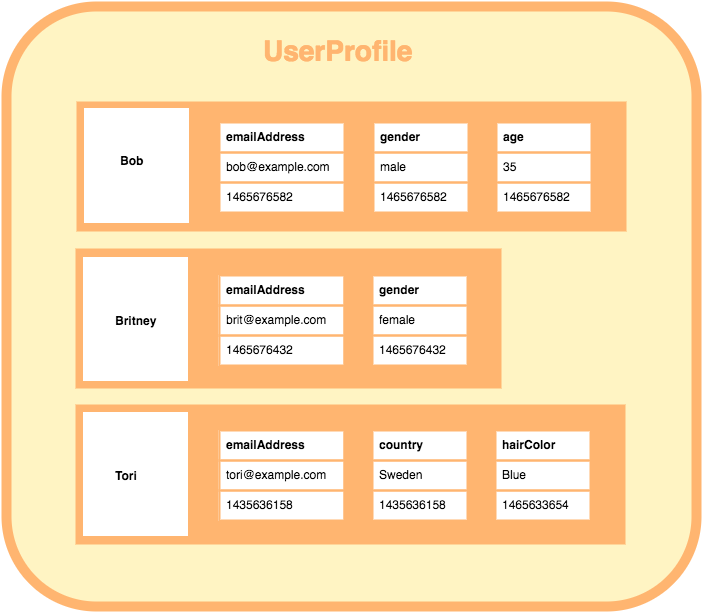
\includegraphics[width=0.75\columnwidth]{img/wide_column_store.png}
    \caption{Example entity relation model \autocite{wideColumnGraphic}}
    \label{fig:cassandra:wide_column}
\end{figure}

\ref{fig:cassandra:wide_column} shows in a graphical representation the structure of a wide column store. The name is the primary key and different people have different columns. The columns with no data are not stored as null but rather not even stored as a whole.

\section{Use-Cases Cassandra}
Cassandra comes with strong benefits over other database systems. These benefits and extra features make it miss some features which one might expect as standard in database systems.
It should be carefully considered whether to use Cassandra or not since it is not the jack of all trades.
One benefit of Cassandra is fast writes which means it can handle a high throughput but the latency might not be too short. These writes include the operations of {INSERT}, {UPDATE} and {DELETE}.
The way Cassandra handles those operations make them equal to a "regular" write operation. This will be explained in section \ref{sec:cassandra:cql}. Another key benefit is high availability. Due to its architecture and depending on the settings, a Cassandra setup can be highly available. Since one of the base assumptions of a distributed system is the expensiveness of inter-node communication, it has an linear horizontal scalability.
The communication between nodes does not increase with the size of node. Due to its distributed nature, the architecture does not rely on a master-slave setting and comes masterless.
Furthermore it can be configured to work with several clusters, globally distributed, which makes for example multicloud Cassandra setups possible.
This means that any client can read from and write to any node. As described previously Cassandra is a wide column store database which results in having a flexible schema where rows can have missing columns that are not stored on disk.
Cassandra has its own query language which is similar \gls{sql} and called \gls{cql}. This makes it easier to use Cassandra if knowledge from \gls{sql} is available.

If any of these points apply to a project or Use-Case, Cassandra is probably a good fit.
But to be sure it is even more important to rule out the cases where Cassandra is not a good fit.
The following paragraph will describe limits of Cassandra. If the use-case needs any of those features, Cassandra will most likely not suffice to fulfill requirements.
First, a single system instance with Cassandra should be avoided. Most of the features and benefits come with multiple node setups. Use-Cases which would need a dozen nodes seem to find a great fit with the distributed storage system.

Equally important is the way data has to be stored and accessed. Due to its architecture, data has to be modeled different in Cassandra. \acrshort{acid} transactions are not possible and tables are fine-tuned for pre defined queries. Those queries should be known early on and not change during use. It is not easily possible to change or extent those queries. Furthermore there are no relations between tables. It is possible to link, connect and reuse IDs but this has to be handled on client side, there are no operations on those IDs available. Additionally column aggregation operations such as \texttt{GROUP BY} are also not possible, since such operations would be very inefficient in a distributed wide column storage.

Having a lot of updates and deletes interspersed with reads slow the system down due to the way of handling requests - just appending data, not changing records and merging them while reading. This has affects on data validation as well. It is not possible to check on write for data uniqueness, constraints or auto increments. \autocite{cassandra_oreilly}

To sum it up there are general Use-Case conditions where Cassandra is a great fit.
In order to make an educated decision the following key-points should fit with the Use-Case and environment:

\begin{itemize}
    \item Large Deployments
    \item High write throughput
    \begin{itemize}
      \item{"High performance at high write volumes with many concurrent client threads"} \autocite{cassandra_oreilly}
    \end{itemize}
    \item Geographical distribution of data and database clients
    \item Different columns per row
\end{itemize}


\section{Data Modeling in Cassandra}  % How to model data (or rather tables)

Compared to other database systems like traditional relational database systems, data modeling is different in Cassandra. Here is a little example to understand the different way of thinking when modeling data for Cassandras wide column data store. \\

Figure~\ref{fig:cassandra:model_data0} shows an example entity relationship diagram of data in the context of a hotel environment. The hotel has the attributes \textit{address}, \textit{phone}, \textit{name} and an \textit{id} as unique primary key. Each hotel has certain amounts of rooms which store information them-self and are connected to other entities.

\begin{figure}[H]
    \centering
    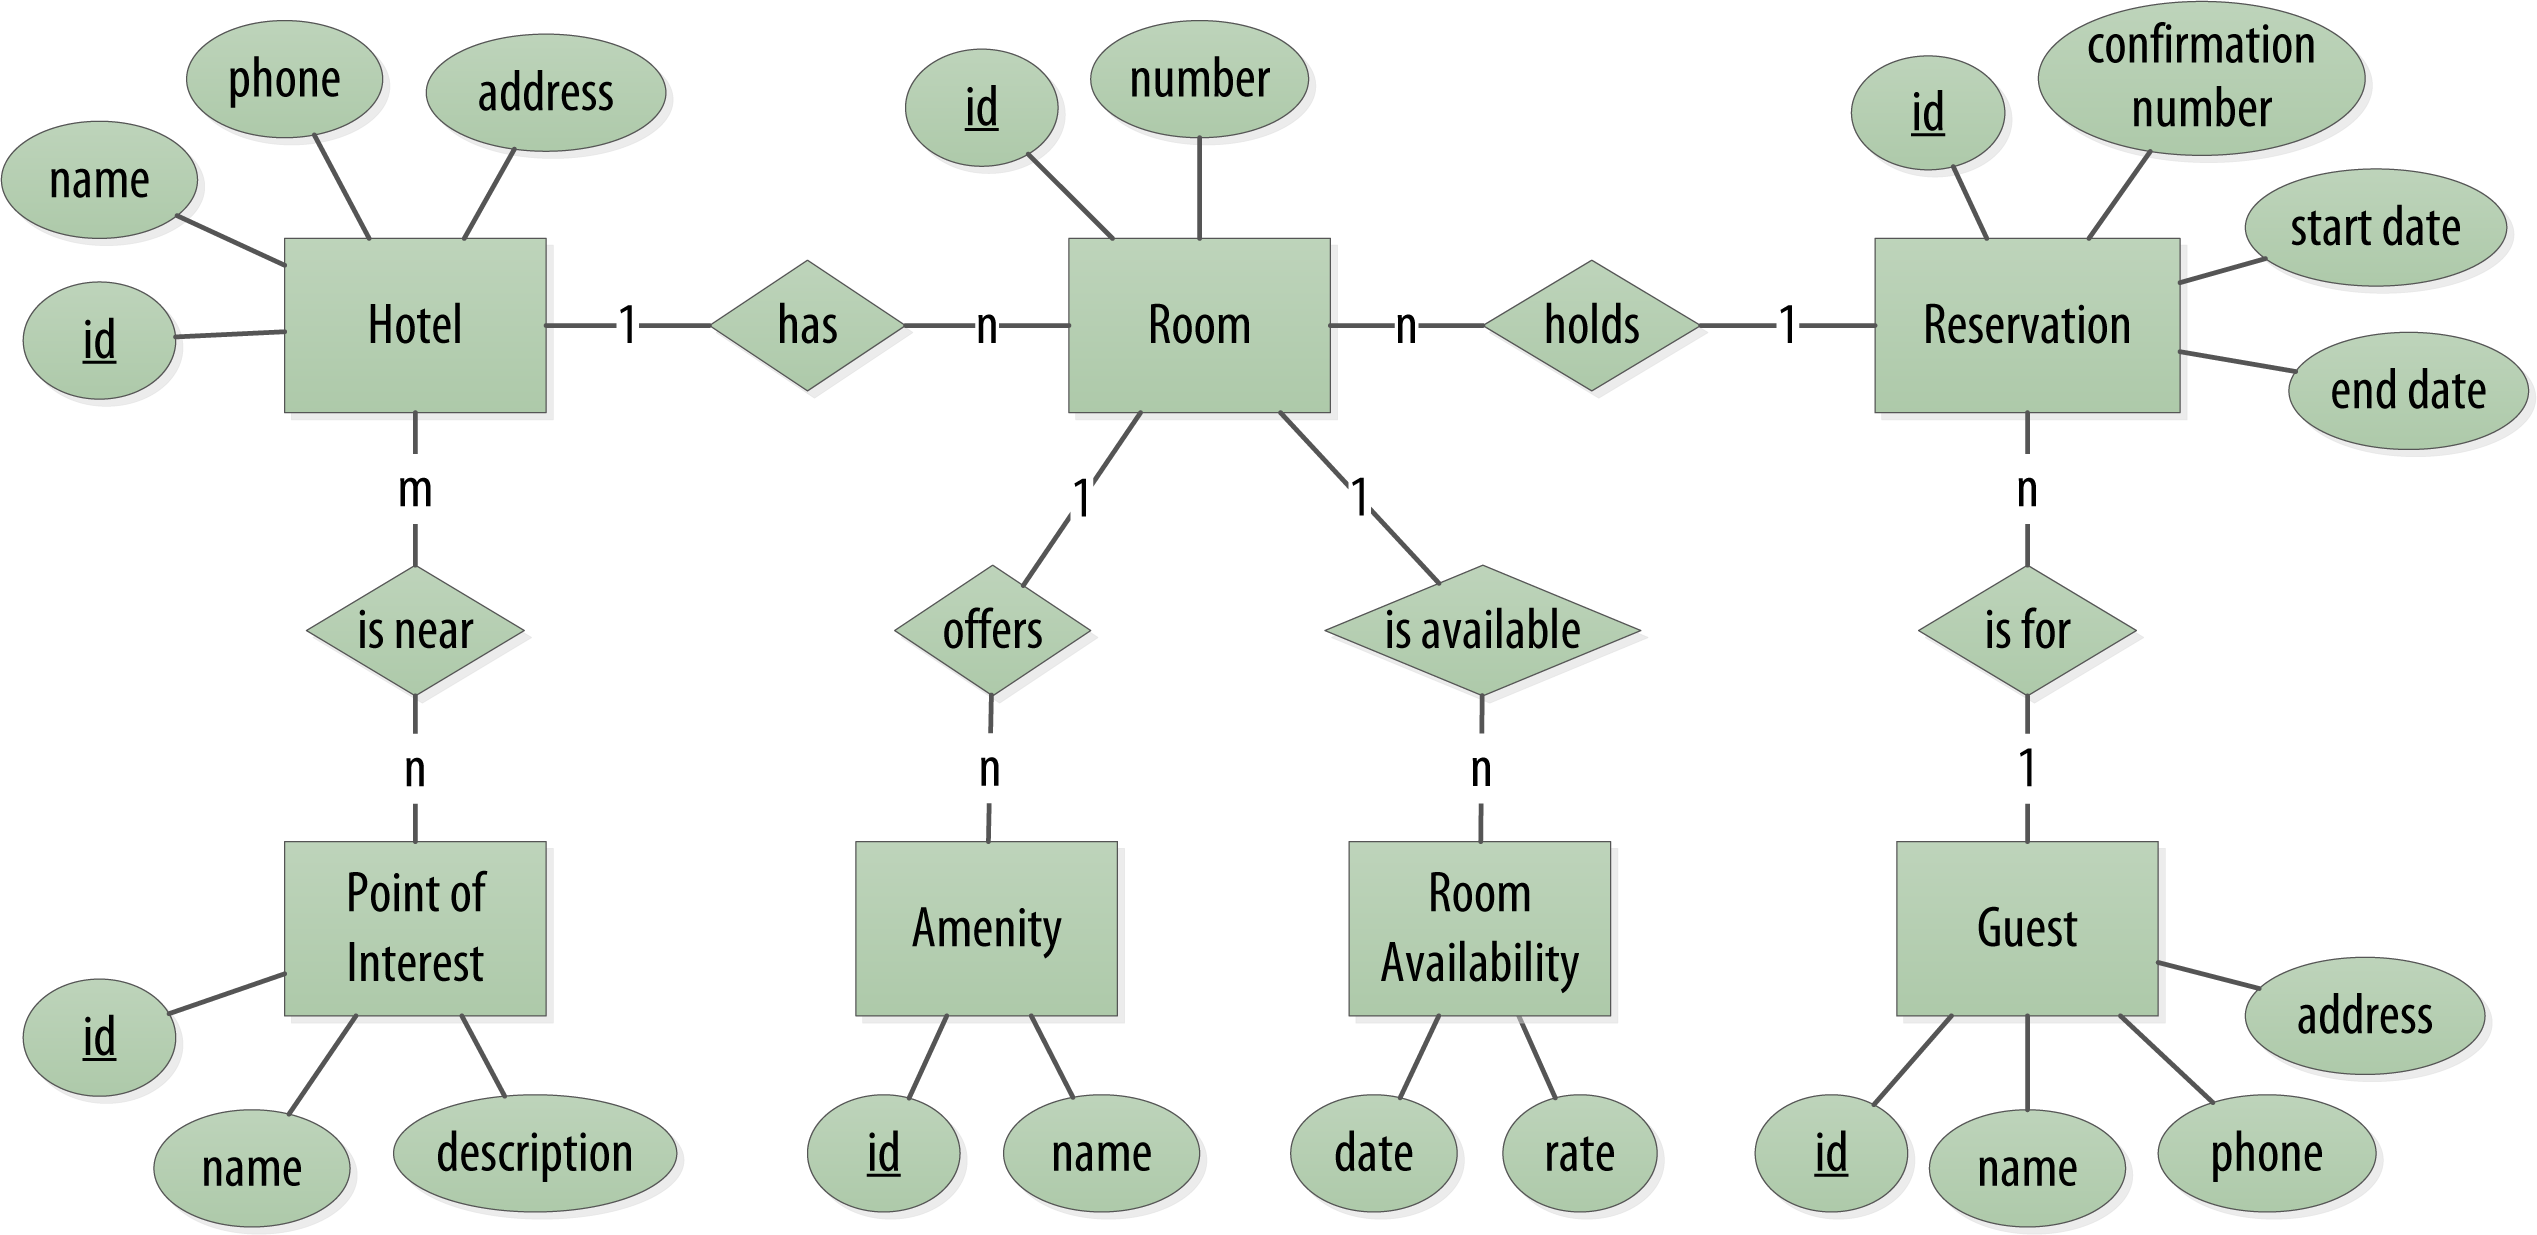
\includegraphics[width=0.75\columnwidth]{img/model_example_entity_relation_step0.png}
    \caption{Example entity relation model \autocite{cassandra_oreilly}}
    \label{fig:cassandra:model_data0}
\end{figure}

In figure~\ref{fig:cassandra:model_data1} an example database model for an relational database of the ERP from figure~\ref{fig:cassandra:model_data0}.
The connections and primary keys previously noted connect now the table to enable complex join queries over multiple tables later on.

\begin{figure}[H]
    \centering
    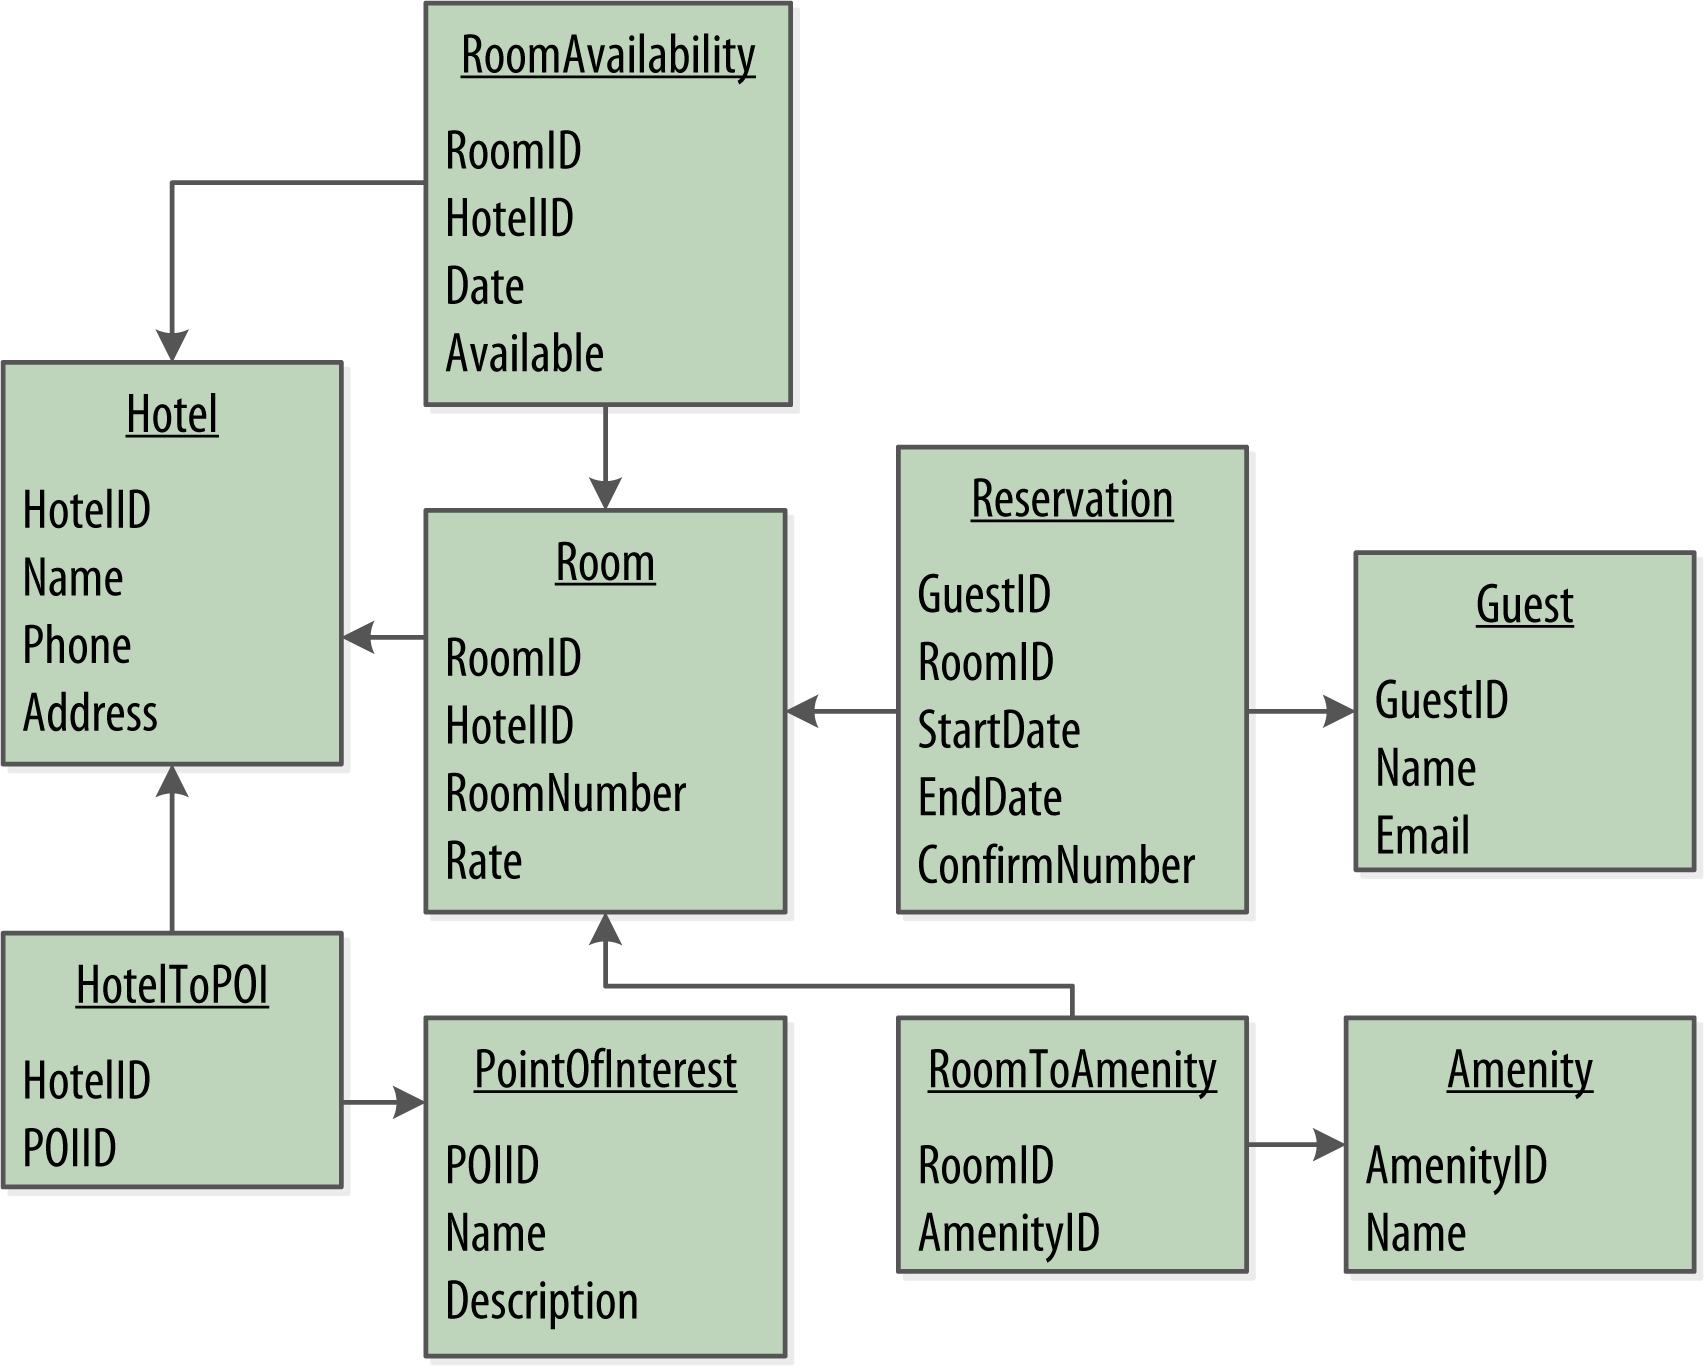
\includegraphics[width=0.75\columnwidth]{img/model_example_rdbms_step1.png}
    \caption{Example RDMBS normalization transition \autocite{cassandra_oreilly}}
    \label{fig:cassandra:model_data1}
\end{figure}

The fundamental difference between those two modeling types is the starting point. In the example above it was all about what data has to be stored and how that data is connected to each other.
In data modeling for Cassandra the queries are the starting points. This means for the architect that they first have to think about queries the database system has to answer.

\begin{figure}[H]
    \centering
    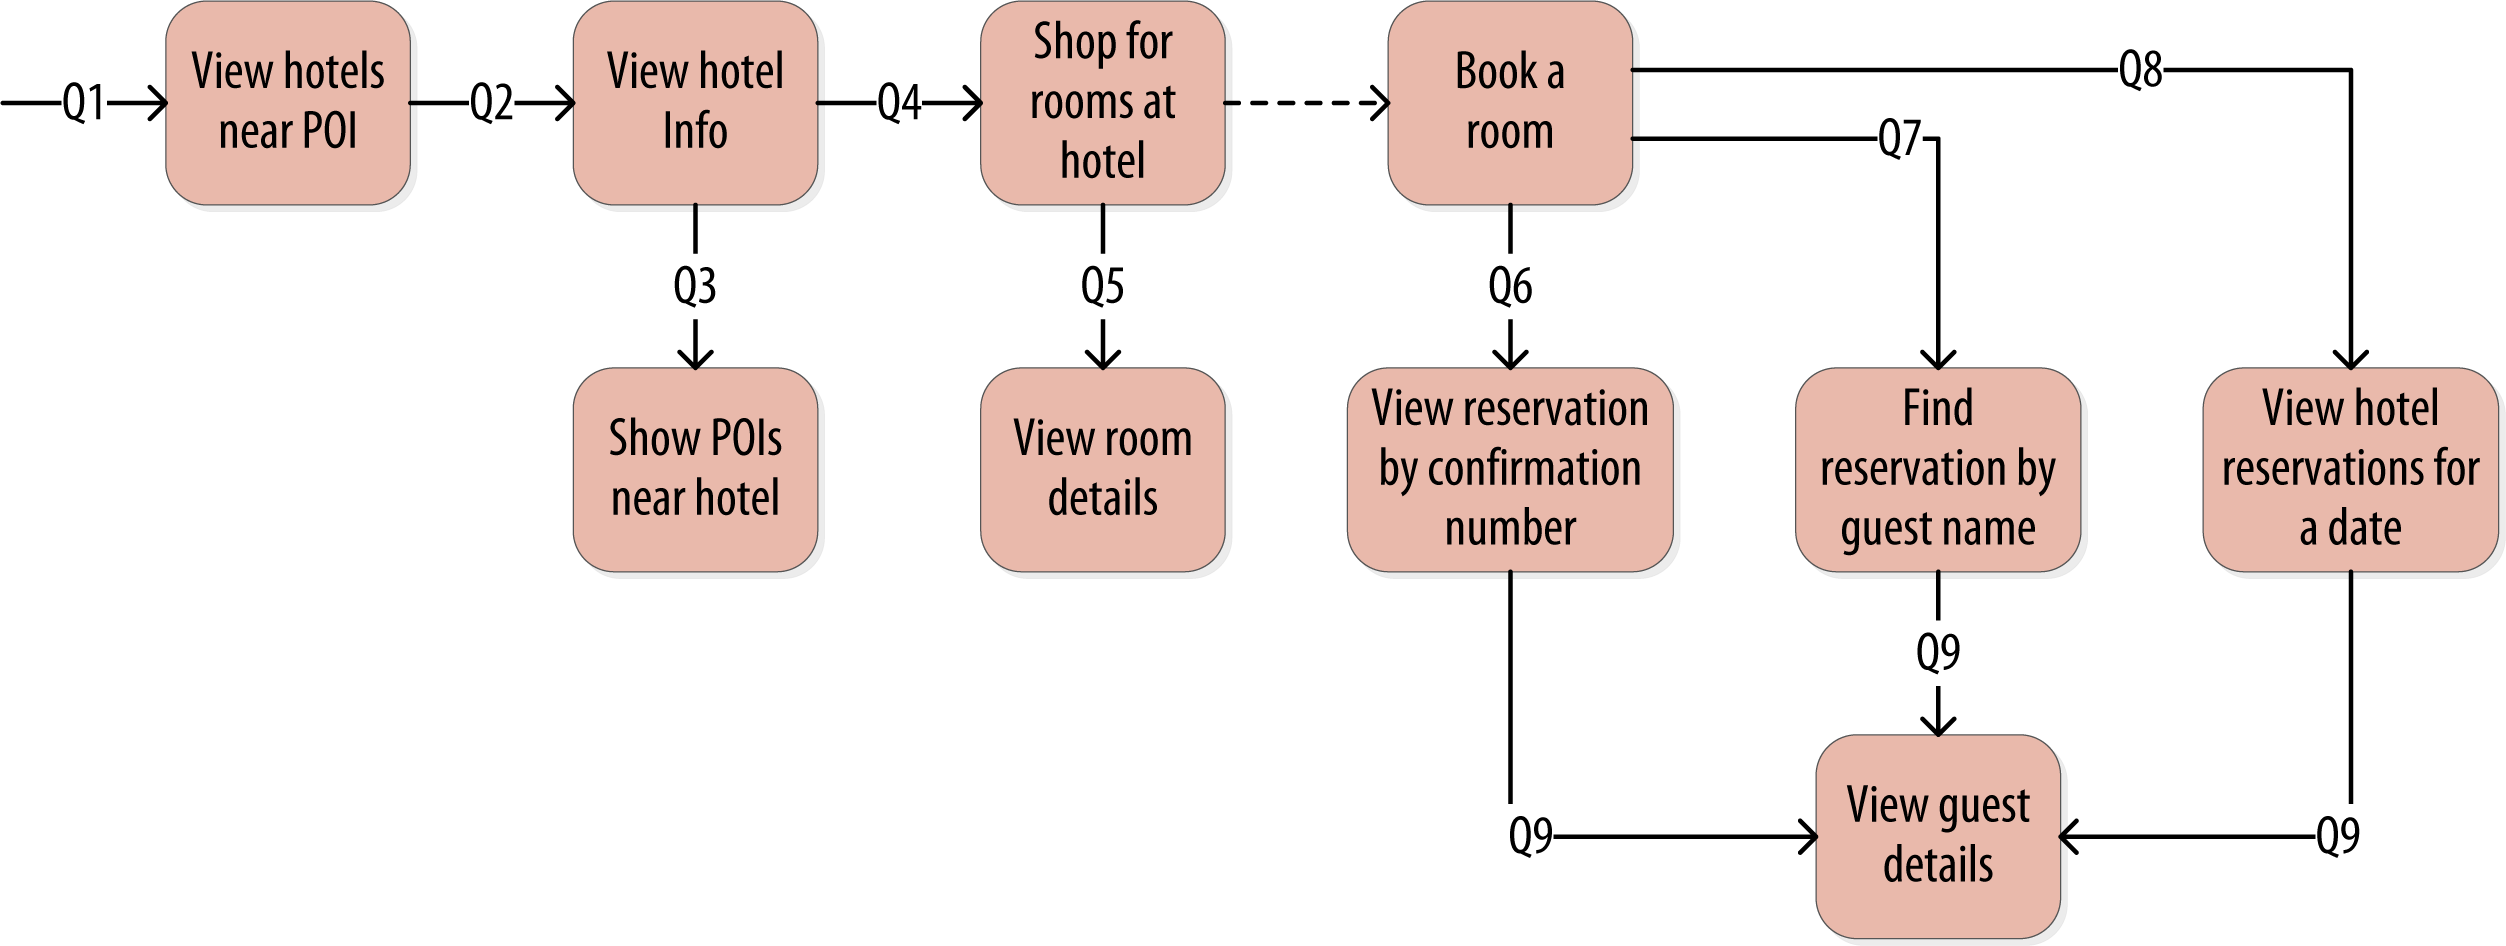
\includegraphics[width=0.75\columnwidth]{img/model_example_queries_step2.png}
    \caption{Planned queries against database system \autocite{cassandra_oreilly}}
    \label{fig:cassandra:model_data2}
\end{figure}

Figure~\ref{fig:cassandra:model_data2} show this circumstance; queries the system later has to answer to. This diagram describes a classical use-case for the hotel environment in which the database would come to work. A user searches for hotels, checks information about it and reserves it.

\begin{figure}[H]
    \centering
    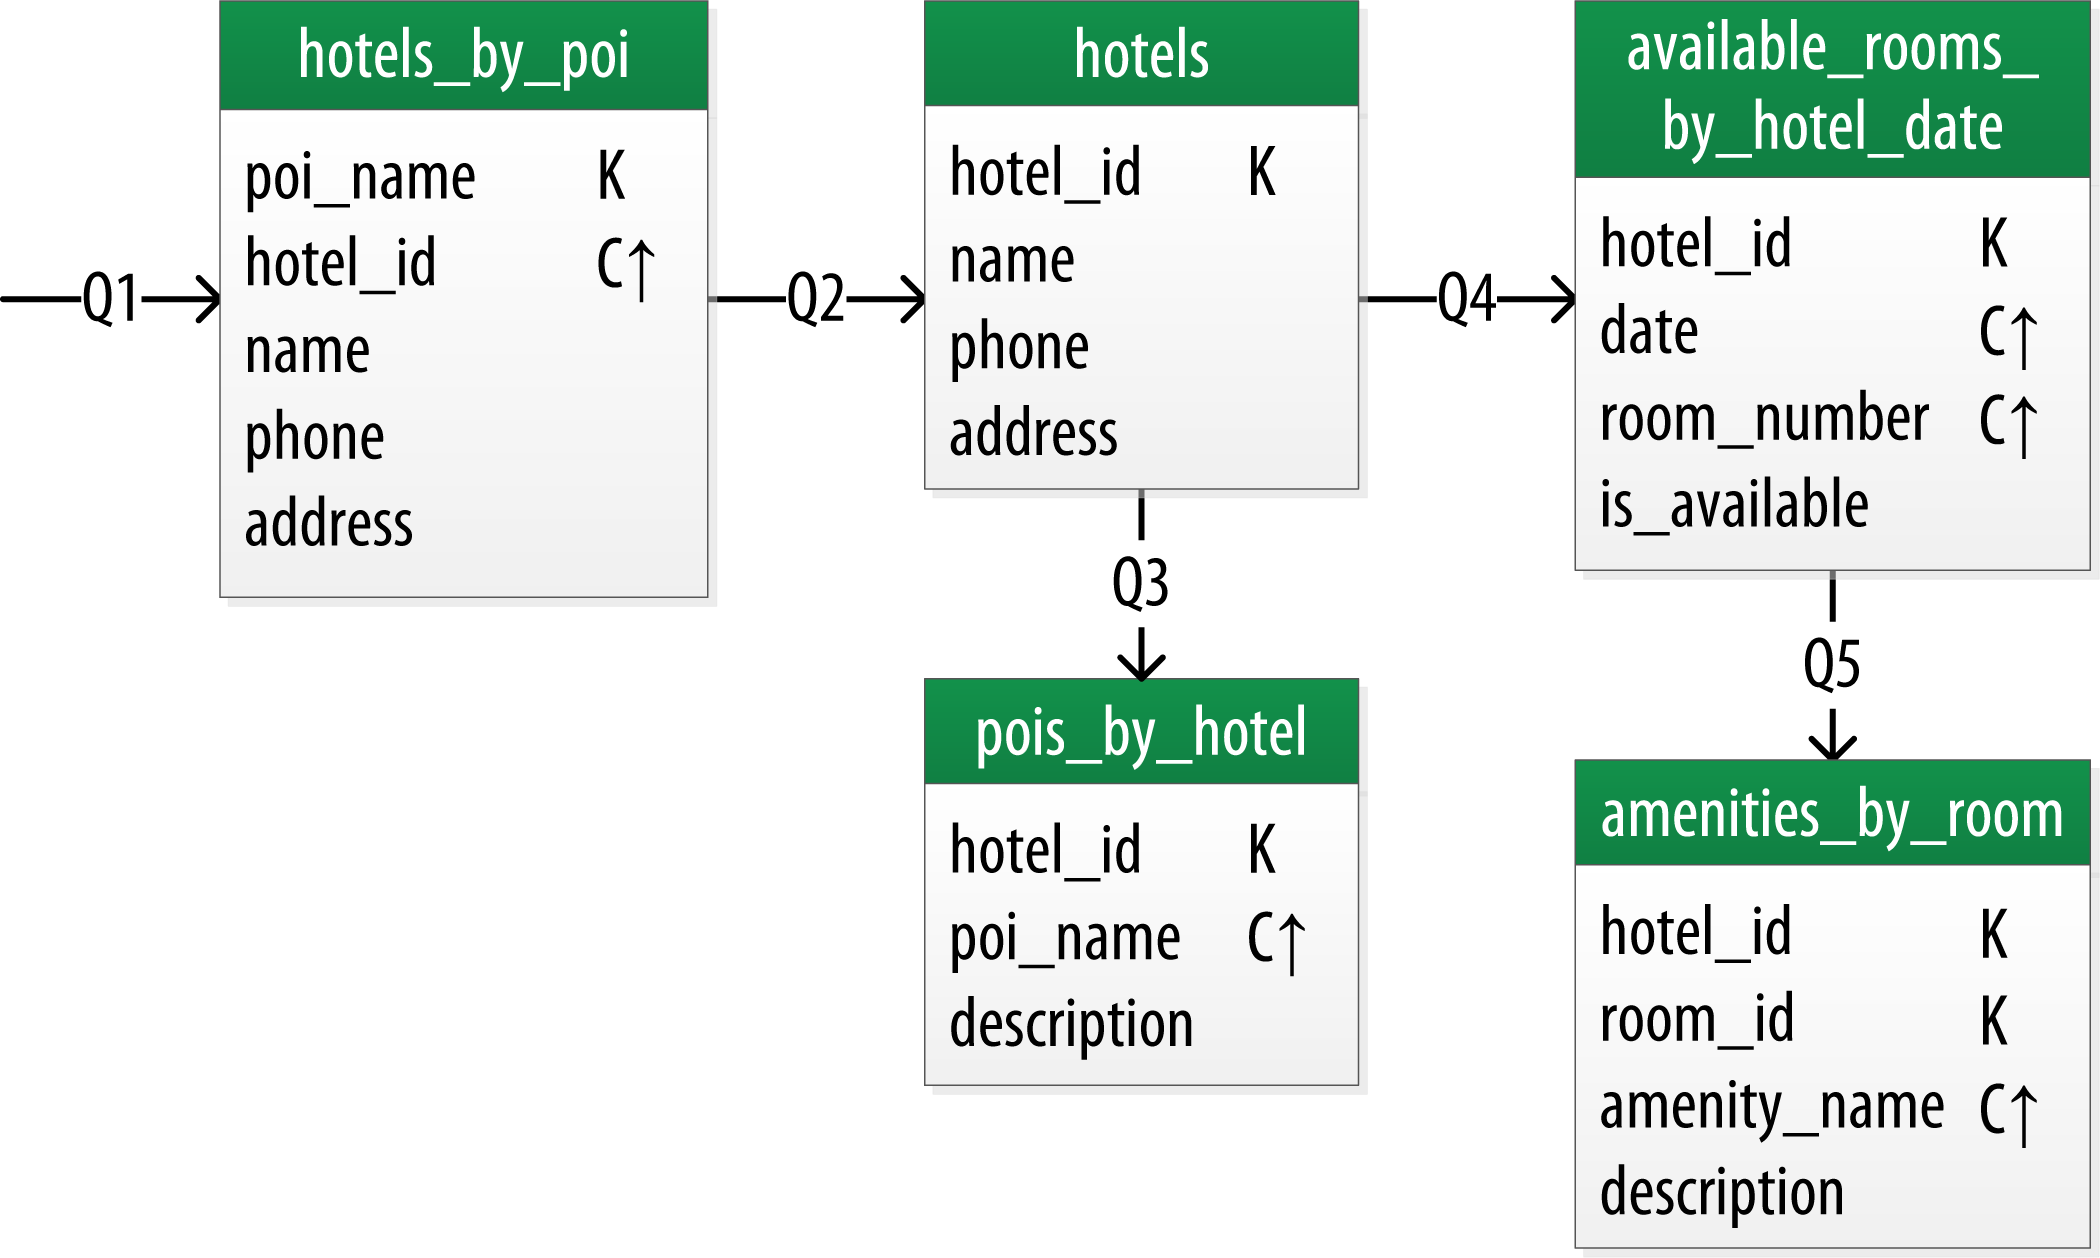
\includegraphics[width=0.75\columnwidth]{img/model_example_chebotko_step3.png}
    \caption{Model and denormalize tables to fit queries \autocite{cassandra_oreilly}}
    \label{fig:cassandra:model_data3}
\end{figure}

Transitioning from the collection of queries in figure~\ref{fig:cassandra:model_data2} to accessible tables, can be seen in figure~\ref{fig:cassandra:model_data3}. It can be seen that data is stored redundantly, available on multiple tables. This does not bother the modeling since queries later on will not use any sort of join operation and be limited onto one table request - which is precisely why data is stored in multiple tables. Each table fulfills one of the queries previously thought of. Furthermore since there is no referential integrity it is possible to store \textit{ids} in tables but the database system does not provide any functionality to make use of and / or connect those \textit{ids}.

In order to properly graph and document this type of modeling, a uniform and new way was proposed to write down data modeling for Cassandra and other similar systems with same needs. \autocite{chebotko2015data}
These diagrams are called Chebotko diagrams and include the way queries are planned. This can be seen in figure~\ref{fig:cassandra:model_data2}.
Out of this table, the diagram can be concluded. Creating to each query an unique table with all necessary information. The arrows with the queries numbers (Q1, Q2 ..) will be kept to keep the context and relation to the previous diagram (\ref{fig:cassandra:model_data3}).
This can be seen in a descriptive example section around figure~\ref{fig:cassandra:chebotko}

\begin{figure}[H]
    \centering
    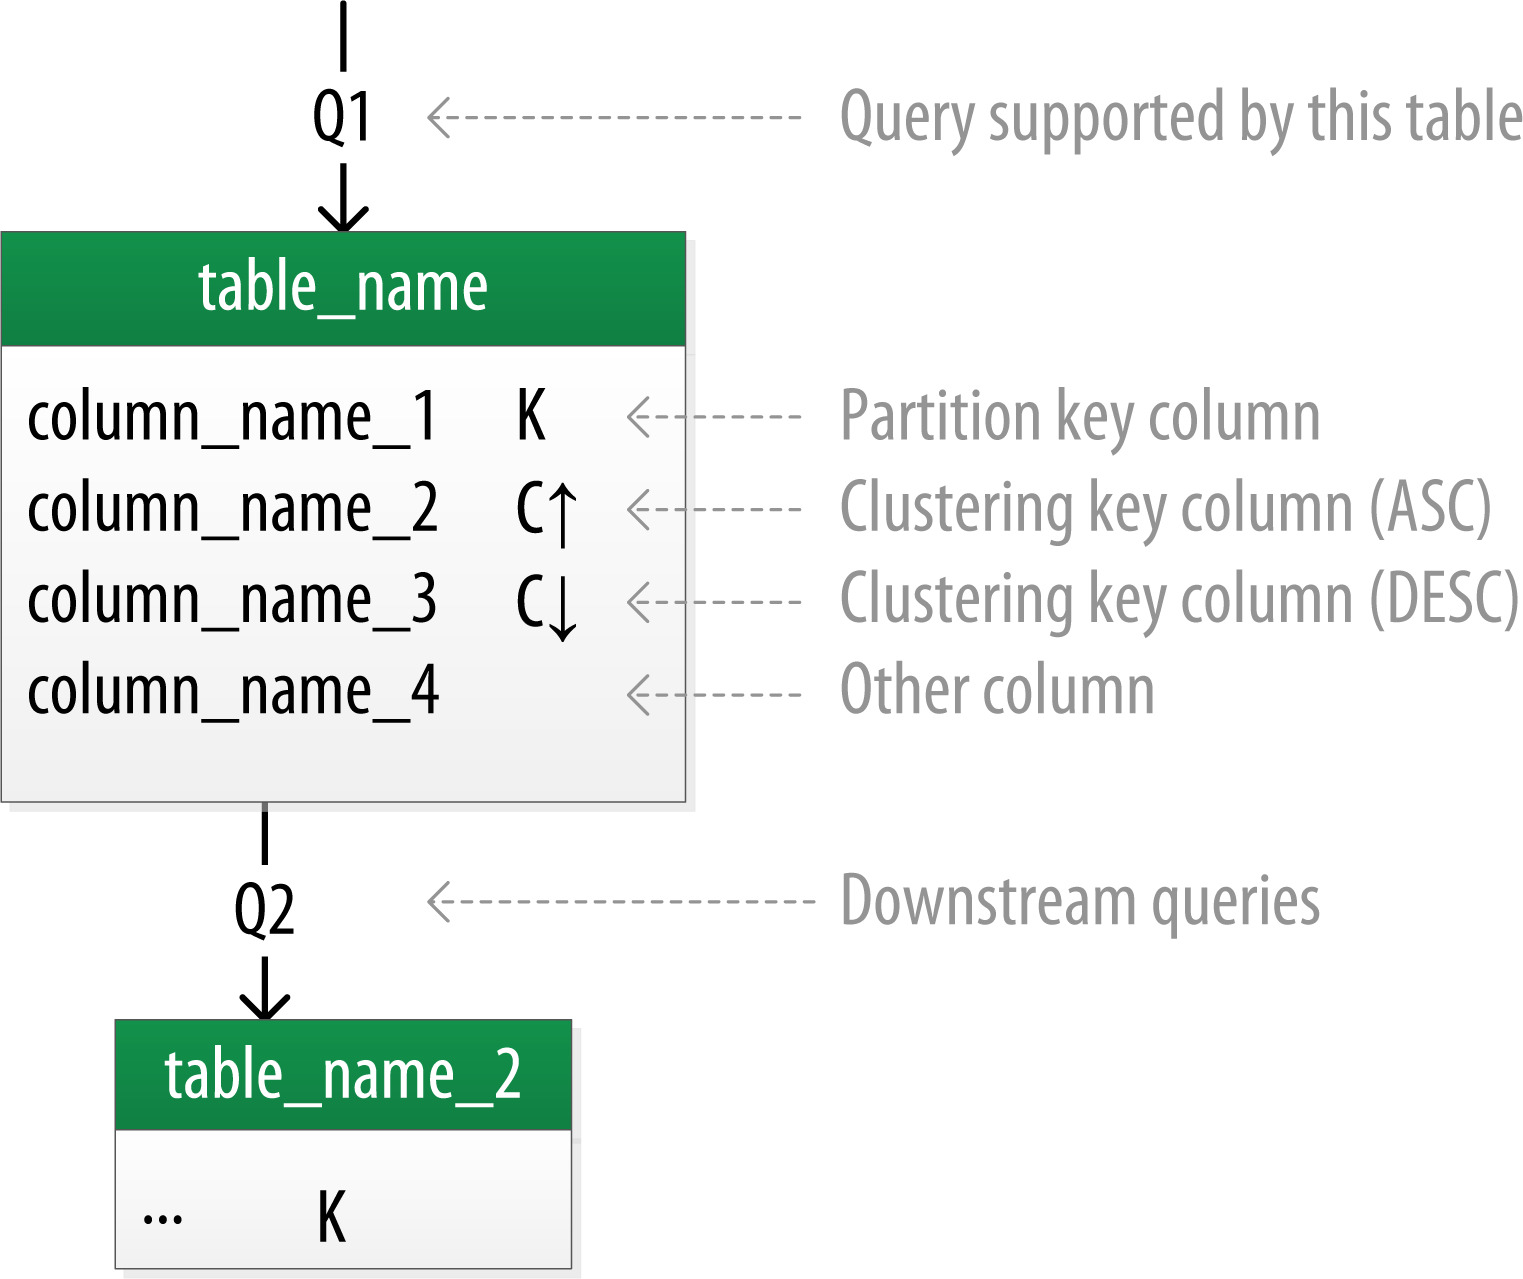
\includegraphics[width=0.75\columnwidth]{img/model_example_primary_key.jpeg}
    \caption{Model and denormalize tables to fit queries \autocite{cassandra_oreilly}}
    \label{fig:cassandra:chebotko}
\end{figure}

\section{Using the Cassandra Query Language} \label{sec:cassandra:cql} % How to use CQL
This section will give a short overview of how to interact with a Cassandra database using \gls{cql}, which is mainly inspired by \gls{sql} \autocite{cqlAlexMeng, newInCQL3, cassandra3cqldocCreateKeystore}.

\subsection {Creating a keyspace}
This similarity becomes clear by looking at how the creation of a keyspace is performed:
\begin{verbatim}
/* Create a new keyspace in CQL */
CREATE KEYSPACE data WITH replication =
    {'class': 'SimpleStrategy', 'replication_factor': 3};

/* Create a new database in SQL */
CREATE DATABASE data;
\end{verbatim}

Hereby the only difference is that instead of creating a database, a keyspace is created and it is possible to specify which replication parameters should be used. What these parameter mean and how they should be used is explained later in section~\ref{sec:CassandraClusterArchitecture} \autocite{cqlAlexMeng}.

\subsection{Creating a table}
After creating a keyspace a table has to be created in order to hold the data. As a database is always part of a keyspace it is either necessary to specify the keyspace in every query or to simple scope every subsequent query into a given keyspace by using the USE query \autocite{cassandra3cqldocUse}:
\begin{verbatim}
USE data;
\end{verbatim}

Using this keyspace a table can be created using the same syntax as in \gls{sql} \autocite{cqlAlexMeng, newInCQL3, cassandra3cqldocCreateTable}:
\begin{verbatim}
CREATE TABLE groups (
   group_name varchar,
   group_location varchar,
   added_date date,
   username varchar,
   PRIMARY KEY (...)
);
\end{verbatim}

Hereby the only difference is how the primary key can be specified:

\begin{figure}[ht]
    \centering
\begin{verbatim}
      partition key       clustering key  clustering key
       |       |                |            |
((groupname, group_location), added_date, username)
\end{verbatim}
    \caption{Parts of a primary key specification in \gls{cql} \autocite{cqlPrimaryKeyDefinition}}
    \label{fig:cassandra:primaryKeyDefinition}
\end{figure}

The first part of the definition will always be the partition key. If it is a compound of several columns they need to be surrounded by parentheses and separated by comma in order to state that they as a whole form the partition key. If necessary the partition key can be followed by several clustering keys. Keep in mind that the data will be ordered first by the first clustering key, after that by the second and so on. This means that an \texttt{ORDER BY} has to first be called on the first clustering key and a second ordering can be done on the subsequent one. It will not be possible to only order by the second or other subsequent clustering keys when not ordering by the first. Any other non-primary key column cannot be used for ordering \autocite{cqlPrimaryKeyDefinition, cassandra3cqldocCreateTable}.

\subsection{Interacting with data}
In order to manipulate Cassandra only provides three possible methods \autocite{lakshman2010cassandra}:
\begin{itemize}
    \item insert(table, key, rowMutation)
    \item get(table, key, columnName)
    \item delete(table, key, columnName)
\end{itemize}
All having in common that the entire primary key has to be specified in order to interact with the data. The only exception hereby is the getting of data where only the partition key has to be specified.

Important to note is that there is no interaction to update a data entry. The reason for that is that as Cassandra is optimized for high write throughput is is very costly to read any data before writing. This means that the update and insert known from \gls{sql} will perform the same action on the data \autocite{cqlAlexMeng, newInCQL3}:
\begin{verbatim}
/* Inserting Data */
INSERT INTO Person (lastname, name, email)
  VALUES ('Doe', 'Jane', 'jane@example.com');

/* Updating Data */
UPDATE Person SET email = 'jane@example.com'
  WHERE lastname='Doe' AND name = 'Jane';
\end{verbatim}

As getting and deleting data is also similar to \gls{sql} there is no need to go into it any further in this section \autocite{cqlAlexMeng, cassandra3cqldocSelect}:
\begin{verbatim}
/* Selecting Data */
SELECT * FROM Person
  WHERE lastname='Doe' AND name = 'Jane';
/* Deleting Data */
DELETE FROM Person
  WHERE lastname='Doe' AND name = 'Jane';
\end{verbatim}

\section{Local reads and writes}
In order to perform the requested changed to the data they have to be written into the database. This section will take a look into how the changes will be written on a single node not taken into account the cluster.

\begin{figure}[ht]
    \centering
    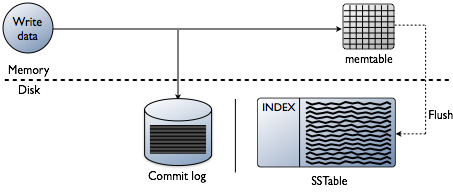
\includegraphics[width=0.75\textwidth]{img/cassandra_local_write.png}
    \caption{Writing data to Cassandra node \autocite{datastaxWriteData}}
    \label{fig:cassandra:writeData}
\end{figure}
In figure~\ref{fig:cassandra:writeData} it can be seen that the write process to Cassandra involves three steps:
\begin{enumerate}
\item \textbf{Write to journal} Hereby the query is simple append to the journal on the disk, making it persistent even if the node goes down. As this action is a simple append it is very fast and leaves the data in a temporal order in the journal.
\item \textbf{Write to memtable} After writing to the journal the change is performed in the memtable putting the data into a Sorted String Table (SSTable). This form is the same form in which the data will be written on disk. Here it is important that only the required data is written if there are any columns not specified it will not be written to the memtable. In contrast to writing \texttt{NULL} to a column which will delete it by setting a tombstone on it (See Appendix \ref{appendix:cassandra:queryExample}).
\item \textbf{Flush to disk when memtable is too big} This allows to simply flush the data and some metadata to the disk when it gets to big for the memory to hold it. Hereby a new data file is created, not touching any of the previously written files, making this action also quite fast as no lookups have to be performed.
\item \textbf{Compacting written datafiles} As writing to disk is only an append and will create a new datafile for every flush, the whole database will be scattered over multiple files with redundant data if entries were written after flushing them to disk. In order to merge these files it is possible to compact the files into one resulting in faster reads later \autocite{cassandraCompactTool}.
\end{enumerate}

After writing the data it also can be read again as shown by figure~\ref{fig:cassandra:readData}:

\begin{figure}[ht]
    \centering
    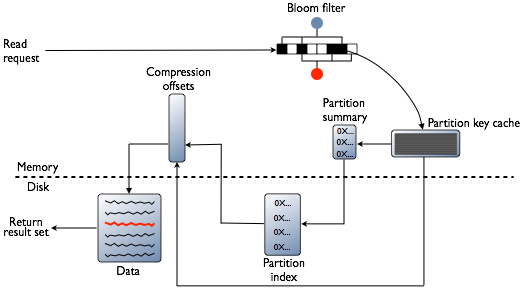
\includegraphics[width=0.75\textwidth]{img/cassandra_local_read.png}
    \caption{Reading data from Cassandra node \autocite{datastaxReadData}}
    \label{fig:cassandra:readData}
\end{figure}
\begin{enumerate}
    \item \textbf{Check caches} First the last query cache will be checked. Returning the data right away if it was requested in the near past.
    \item \textbf{Check memtable} If not found in the caches the memtable will be checked whether it has the most recent activities on the requested data.
    \item \textbf{Find SSTable and location} If no entry was found in the memtable the data on disk will be checked by firstly determining in which memtable dump the dataset will be and then retrieving it from there. For a detailed overview of this take a look at figure \ref{fig:cassandra:readData}
    \item \textbf{Merge with memtable} If it was necessary to retrieve the data from disk the data will be written to the memtable to allow later queries on the same data to succeed earlier.
\end{enumerate}

\section{Cluster Architecture}\label{sec:CassandraClusterArchitecture}  % How the cluster works
Which node has a certain piece of data is not determined by a master server. Any node has the ability to determine where a particular piece of data is or must be stored just by hashing the partition key of a row. The result of that calculation is called a token. All nodes are placed somewhere on a \textit{token ring} (see figure~\ref{fig:cassandra:tokenring}) and store the data of the tokens they are assigned to.\autocite[2]{lakshman2010cassandra} \autocite[209,210]{DeCandia2007Dynamo}

\newcommand{\Ray}{3cm}
\begin{figure}[ht]
  \centering
  \begin{tikzpicture}
    % Nodes on the circles
    \node[circle,minimum width=2cm,minimum height=1cm,draw,name path=n1] (Node A) at (90:\Ray) {A};
    \node[circle,minimum width=2cm,minimum height=1cm,draw,name path=n2] (Node B) at (0:\Ray) {B};
    \node[circle,minimum width=2cm,minimum height=1cm,draw,name path=n3] (Node C) at (270:\Ray) {C};
    \node[circle,minimum width=2cm,minimum height=1cm,draw,name path=n4] (Node C) at (180:\Ray) {D};

    % Circle the nodes are placed on
    \path[name path=c] circle (\Ray);
    \path[name intersections={of=n1 and c,name=i1},
          name intersections={of=n2 and c,name=i2},
          name intersections={of=n3 and c,name=i3},
          name intersections={of=n4 and c,name=i4}
         ];

    % Arrows between the nodes
    \begin{scope}
      \pgfsetarrowsend{Stealth[scale=1.5]}

      \pgfpathmoveto{\pgfpointanchor{i1-2}{center}}
      \pgfpatharcto{\Ray}{\Ray}{0}{0}{0}{\pgfpointanchor{i2-1}{center}}
      \pgfusepath{draw}

      \pgfpathmoveto{\pgfpointanchor{i2-2}{center}}
      \pgfpatharcto{\Ray}{\Ray}{0}{0}{0}{\pgfpointanchor{i3-1}{center}}
      \pgfusepath{draw}

      \pgfpathmoveto{\pgfpointanchor{i3-2}{center}}
      \pgfpatharcto{\Ray}{\Ray}{0}{0}{0}{\pgfpointanchor{i4-2}{center}}
      \pgfusepath{draw}

      \pgfpathmoveto{\pgfpointanchor{i4-1}{center}}
      \pgfpatharcto{\Ray}{\Ray}{0}{0}{0}{\pgfpointanchor{i1-1}{center}}
      \pgfusepath{draw}
    \end{scope}

    % Labels on arrows
    \node[fill=white] at (45:\Ray) {0 to 63};
    \node[fill=white] at (135:\Ray) {64 to 127};
    \node[fill=white] at (225:\Ray) {128 to 191};
    \node[fill=white] at (315:\Ray) {192 to 255};
  \end{tikzpicture}
  \caption{Token Ring}
  \label{fig:cassandra:tokenring}
\end{figure}

The tokens from the node's location to the next node belong to it. That means if the hashing of a partition key results in a token between 0 and 63 the data will be written to or read from node A. Keep in mind: This doesn't however mean that this node is \textit{in control} of that data - when replication is configured all replicas are equal. The node with that token is just the starting point to determine the first of the replicas.

\paragraph{Replication} To ensure that all data continues to be available even if some nodes go down Cassandra replicates the data in the cluster. Replication can be defined for each keyspace when it is created. There is a simple strategy and a network topology aware strategy. \autocite{datastax_replication} \\
The \texttt{SimpleStrategy} places the $n$ replicas of a piece of data on the next $n-1$ nodes\footnote{The first node that holds the data also counts as a replica.} located clockwise on the ring after the node with the token. \autocite[3]{lakshman2010cassandra} \\
The \texttt{NetworkTopologyStrategy} strategy tries to be smart about the physical placement of replicas. It needs to be taught about in which datacenter and rack the nodes are located. To avoid losing data when an entire rack or datacenter fails this strategy prefers to spread it out.
It is recommended to use this strategy in production, unless all nodes are in a single rack, where both strategies are equivalent.

\paragraph{Rebalancing}

When a new node is added or a node is removed it is likely that the distribution of nodes on the ring becomes imbalanced. When the ring is imbalanced nodes are responsible for different amounts of data and experience different amounts of load. Since nodes are recommended to be of the same performance level\footnote{Or be balanced by dividing them up into virtual nodes according to performance} this is not optimal. Some nodes are overloaded and others underutilized.
To balance the ring the nodes are moved to equidistant positions on the ring. When this happens data is bound to be assigned to a new owner node - that data will be moved. \autocite{datastax_balancing}
The hash function used to transform partition key into is a so called \textit{consistent hash function}. The difference from a regular (cryptographically secure) hash function is that the output wraps around and thus can be represented as a ring. It also has the property that it minimizes the amount of shifting data that is necessary when a node is added or removed. \autocite{karger1997consistent}

Figure~\ref{fig:cassandra:rebalancing} visualizes an imbalanced ring and how the green nodes can be repositioned.


\begin{figure}[ht]
  \centering
  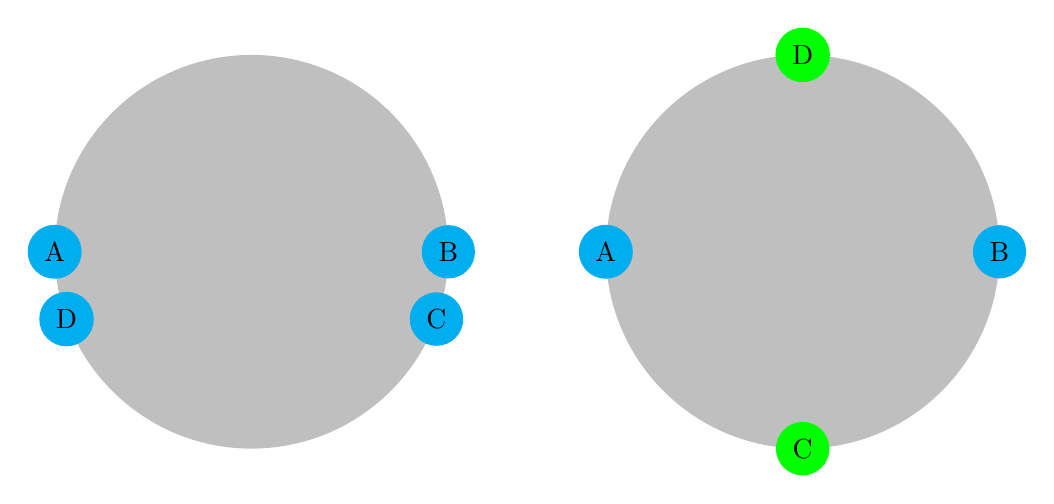
\begin{tikzpicture}
    % Circle
    \fill[fill=black!25] (2.5, 0) arc (0:360:2.5);
    \node[circle,fill=cyan] at (180:2.5) {A};
    \node[circle,fill=cyan] at (0:2.5) {B};
    \node[circle,fill=cyan] at (-20:2.5) {C};
    \node[circle,fill=cyan] at (200:2.5) {D};

    % Legend
    \begin{scope}[shift={(7,0)}]
      \fill[fill=black!25] (2.5, 0) arc (0:360:2.5);
      \node[circle,fill=cyan] at (180:2.5) {A};
      \node[circle,fill=cyan] at (0:2.5) {B};
      \node[circle,fill=green] at (270:2.5) {C};
      \node[circle,fill=green] at (90:2.5) {D};
    \end{scope}
  \end{tikzpicture}
  \caption{Rebalancing}
  \label{fig:cassandra:rebalancing}
\end{figure}

Nodes A and B can stay at their location, C and D are repositioned. C is moved further along the ring in a clockwise direction. It gives much of the data it was previously responsible to B and takes all of D's data. D is moved past A and takes approximately half of its data.

\paragraph{Virtual Nodes}

By default each node is placed on the ring just once, when using virtual nodes they each can be placed on the node multiple times. This brings four advantages: \autocite{datastax_vnodes, yelp_balancing}

\begin{itemize}
  \item Nodes can occupy a specified proportion of the ring
  \item Tokens are automatically calculated and assigned to nodes $rightarrow$ No manual rebalancing
  \item Data hotspots on the ring are handled my multiple nodes
  \item Rebuilding of replacements is faster
\end{itemize}

1. When nodes have different processing capabilities and disk space that performance difference should be taken into account so that all nodes receive load which is proportional to their performance. With virtual nodes enabled a node can be assigned any number of tokens. Not the absolute number of tokens of an individual node is relevant it only has an effect on how much of the ring it occupies on relation to the others.  \\
2. Without using virtual nodes the tokens for each node have to be calculated manually and assigned to each node. Cassandra also automatically rebalances the ring whenever a new node joins or a node leaves. \\
3. When data partitioning was done poorly or the data happens to cluster around a particular token range the node responsible for that data receives disproportionately much load. Virtual nodes remedy that because they not only make the individual partitions smaller but they also make any single note responsible for multiple areas on the ring. \\
4. When a node goes down and a replacement is brought up. This replacement needs the data of the node it replaced. If the replication factor is three it needs data from three different partitions. Without virtual nodes this can come from up to $3\cdot(3-1)=6$ different replicas. When using virtual nodes the partitions the same amount of data is spread across more nodes and thus the replication can transfer data from more nodes at once. If each node is split into $k$ virtual nodes it can replicate from $k$ times more replicas.

See figure~\ref{fig:cassandra:vnodes} for a visualization.

\begin{figure}[ht]
  \centering
  \begin{tikzpicture}
    % Circle
    \draw[line width=1.5mm] (\Ray, 0) arc (0:360:\Ray);

    % Nodes on the circle
    \foreach \x [count=\p] in {0,...,2} {
      \node[circle,draw,minimum size=1cm,fill=orange] at (90-\x*120-0*30:\Ray)
        {\pgfmathparse{1+4*\x}\pgfmathprintnumber{\pgfmathresult}};
      \node[circle,draw,minimum size=1cm,fill=cyan] at (90-\x*120-1*30:\Ray)
        {\pgfmathparse{2+4*\x}\pgfmathprintnumber{\pgfmathresult}};
      \node[circle,draw,minimum size=1cm,fill=yellow] at (90-\x*120-2*30:\Ray)
        {\pgfmathparse{3+4*\x}\pgfmathprintnumber{\pgfmathresult}};
      \node[circle,draw,minimum size=1cm,fill=black!25] at (90-\x*120-3*30:\Ray)
        {\pgfmathparse{4+4*\x}\pgfmathprintnumber{\pgfmathresult}};
    };

    \node[circle,draw,minimum size=1cm,fill=orange,label=right:{Node A}] at (2*\Ray, 1.875) {};
    \node[circle,draw,minimum size=1cm,fill=cyan,label=right:{Node B}] at (2*\Ray, 0.625) {};
    \node[circle,draw,minimum size=1cm,fill=yellow,label=right:{Node C}] at (2*\Ray, -0.625) {};
    \node[circle,draw,minimum size=1cm,fill=black!25,label=right:{Node D}] at (2*\Ray, -1.875) {};
  \end{tikzpicture}
  \caption{Virtual Nodes}
  \label{fig:cassandra:vnodes}
\end{figure}

\subsection{Distributed writes and reads (CAP Theorem)} \label{subsec:cassandra:cap}

Cassandra has a masterless architecture; no single node controls any particular piece of data \autocite[5]{lakshman2010cassandra}\footnote{Unless explicitly configured to do so}. A consequence is that a client can run queries against any node of the cluster. In practice the client determines, either by some heuristic of proximity/latency or a round-robin algorithm, which node to use.
For one query that particular node becomes the \textit{coordinator node}; it coordinates the execution and distribution of that query.
First it hashes the partition key of the data to obtain the token and finds the node responsible for it. By using the replication strategy it can find out which replicas are responsible for that data as well. \\
When executing a read query the coordinator asks all replicas\footnote{A replica is every node responsible for that piece of data - the one determined by hashing as well as the others determined by replication strategy.} for the data. When more than \texttt{CL.read} replicas have answered the client is given an answer. When the replicas don't agree on the value of the data the client is sent the newest copy. Once all answers have come in the replicas with outdated information are sent a message on how to update their data, this is called a \textit{read repair}. \autocite{cassandra_distributed_read} \\
When executing a write query the coordinator sends the write request to all responsible replicas. If a replica is not currently available the coordinator logs the request and retries it later when the replica is back up  - this is called a \textit{hinted handoff}\autocite[6,7]{cassandraInCAPtheorem}. After more than \texttt{Cl.write} replicas have responded that they successfully completed the write the client is given a successful response. \autocite{cassandra_distributed_write}

For an explanation of the consistency levels \texttt{CL.read} and \texttt{CL.write} see section~\ref{subsec:cassandra:cap}.

In short, the process looks like this:

\begin{enumerate}
  \item Client sends query to any node
  \item That node becomes coordinator
  \item Coordinator determines tokens by hashing
  \item Coordinator sends write or read requests to all replicas determined by replication strategy
  \item For writing
    \begin{enumerate}
      \item Return success to client when more than \texttt{CL.write} nodes have acknowledged
      \item Write \textit{hinted handoff} to log for nodes that are currently unavailable
    \end{enumerate}
  \addtocounter{enumi}{-1}  % Both writing and reading should have the same number
  \item For reading
    \begin{enumerate}
      \item Return newest response when more than \texttt{CL.read} nodes have responed
      \item Send \texttt{read\_repair} to nodes with outdated data
    \end{enumerate}
\end{enumerate}

This process is also illustrated by figure~\ref{fig:cassandra:replication}.
The client queries node 4 which becomes the coordinator and then itself queries all replicas (1, 8 and 11).
When node 1 answers the default consistency level of \texttt{ONE} is satisfied and an answer is returned to the client.

\begin{figure}[ht]
  \centering
  \begin{tikzpicture}
    % Circle
    \filldraw[fill=cyan] (\Ray, 0) arc (0:360:\Ray);

    % Nodes on the circle
    \foreach \x [count=\p] in {0,...,11} {
      \def\nodeColor{orange}
      \ifnum \p=1
        \def\nodeColor{green}
      \fi
      \ifnum \p=8
        \def\nodeColor{green}
      \fi
      \ifnum \p=11
        \def\nodeColor{green}
      \fi
      \ifnum \p=4
        \def\nodeColor{yellow}
      \fi
      \node[circle,draw,scale=0.75,fill=\nodeColor] (\p) at (90-\x*30:\Ray) {\p};
    };

    % Arrows between the nodes
    \draw [->,thick] (4) to[bend right=10] (1);
    \draw [<-,thick,draw=red] (4) to[bend left=10] (1);
    \draw [->,thick, dashed, blue] (4) -- (11);
    \draw [->,thick, dashed, blue] (4) -- (8);

    % Client plus its arrows
    \node[fill=cyan,draw,minimum width=1.5cm,minimum height=1cm,rounded corners=.1cm] (Client) at (2*\Ray, 0) {Client};
    \draw [->,thick,draw=red] (4) to[bend right=10] (Client);
    \draw [<-,thick] (4) to[bend left=10] (Client);

    % Legend
    \node[circle,draw,scale=0.75,fill=yellow,label=right:{Coordinator Node}] (coordinatorLegend) at (2.5*\Ray, 0.5) {N};
    \node[circle,draw,scale=0.75,fill=green,label=right:{Replica}] (replicaLegend) at (2.5*\Ray, -0.5) {N};
  \end{tikzpicture}
  \caption{Replication}
  \label{fig:cassandra:replication}
\end{figure}

\paragraph{Tuning Consistency} By default writes and reads need to be acknowledged by only a single replica. Usually data is configured to be replicated over multiple nodes. The result is that queries to Cassandra are highly available - any particular node can fail and the request will receive a successful response. This comes at the cost that not all replicas always have the same data - a lack of consistency. \\
Because different applications have different requirements of availability and consistency Cassandra offers several parameters to adjust its alignment on that spectrum.

One of those is the consistency level. As previously mentioned in this section it determines how many nodes have to acknowledge a request until enough nodes have acknowledged completion. Consistency level for reading and writing are abbreviated as \texttt{CL.read} and \texttt{CL.write} respectively.

Cassandra offers these, but not limited to these, options. \autocite{datastax_consistency_level}

\begin{itemize}
  \item \texttt{ALL} replicas
  \item \texttt{QUORUM}: A majority of the replicas: half + 1
  \item \texttt{THREE} replicas
  \item \texttt{TWO} replicas
  \item \texttt{ONE} replicas (default)
  \item \texttt{ANY}: Only writing - At least one replica or a logged \textit{hinted handoff} if all are unavailable
\end{itemize}

In addition to these levels Cassandra also offers others that also take into account how nodes are distributed into different datacenters. \\
For each query, but usually an entire client session, the consistency level can be chosen.

The \texttt{ALL} level yields the highest consistency. Only when all replicas have responded the response is given to the client. That means either all were updated or all were asked for their current dataset. Thus there is no uncertainty about what the result is - all replicas must agree. The \texttt{ANY} consistency level is the least consistent. The data does not have to be fully written to any SSTable, memtable or even commit log of a replica - a simple \textit{hinted handoff} on the coordinator is enough. \autocite[6,7]{cassandraInCAPtheorem}

\paragraph{Replication Factor} Whenever creating a keyspace you have to configure its replication strategy. Whatever strategy you choose you have to determine how often you want a piece of data to be replicated. If you go with the lowest possible value of 1 the failure of any node will inevitably lead to data loss (read and write failures). Increasing the replication factor means that more nodes can fail while requests can still be properly responded to - this means increased availability. It will, however, also mean that the additional replicas can get out of sync, which lowers the consistency. \autocite[3]{lakshman2010cassandra}

We see that by default Cassandra is highly available and only eventually consistent but it can be gradually tuned to being highly consistent but more prone to failure. \autocite[2,3]{cassandraInCAPtheorem}

\section{Setup and Configuration}  % Setup
Cassandra is designed to be run in a cluster of multiple machines. That has to be kept in mind, even when setting up a single instance. That single instance would form a single node cluster. This makes manual configuration unavoidable - every node needs to know how to join the cluster.
For the purpose of joining the cluster each node is configured with a list of \textit{seed nodes}. When starting up for the first time it asks those nodes about the state of the ring and the new node is assigned a place on the ring. After joining the cluster is complete and the distinction of \textit{seed nodes} is no longer relevant - all nodes are equally important.
When a new node was added it is responsible for a chunk of the data the others were previously responsible for. They do not remove that, now unnecessary, data on their own - to do so run \texttt{nodetool cleanup} on each of the old nodes.

A simple but sufficient\footnote{The other settings can be left at their defaults.} configuration of the first node would look like shown in listing~\ref{lst:cassandra:first_node_config}. \autocite{cassandra_config}

\begin{listing}[ht]
  \begin{minted}{yaml}
# Open socket on this address
listen_address: "192.168.0.2"
# Tell other nodes its reachable on this address
broadcast_address: "3.14.1.59"

seed_provider:
  - class_name: org.apache.cassandra.locator.SimpleSeedProvider
    parameters:
      - seeds "3.14.1.59"

# Enable client communication
start_native_transport: true
  \end{minted}
  \caption{Configuration of first node}
  \label{lst:cassandra:first_node_config}
\end{listing}

For the masterless cluster to function all nodes need to be able to reach all other nodes. This is trivial if all are in the same subnet of the network. Then they can just reach each other by their IP addresses.
When they are in different subnets however they each have a private (local to their subnet) and public (inter subnet) address. This is very often the case in public cloud offerings. There are just not enough addresses available to give every node a public one.
Cassandra needs to know two things:
1. On what address to listen for oncoming TCP connections. That's what \texttt{listen\_address} is for. This is the local/private address.
2. What address to tell other nodes it's reachable under. This is set by \texttt{broadcast\_address} and it is the public address that all other nodes must be able to reach.
Therefore in a local network (with no address translation between the nodes) \texttt{listen\_address} and \texttt{broadcast\_address} are set to the same value.

In order to create a single cluster instance the node has to have its seed set to containing only its own address. Since it doesn't need to listen on a public or even private IP this should, in most cases, be \texttt{localhost}.
The first node of a cluster can be thought of as such a single instance node until others join.

In order for additional nodes to join the cluster configure them analogous to the first, changing the address values but keeping the seed list.
Upon starting them they will automatically communicate with the seed and join the cluster.

\paragraph{More configuration} Cassandra has many more parameters that we are not going to mention here. They can be used to adjust everything from performance tuning, architectural changes or increasing security.
To use virtual nodes explained in section~\ref{sec:CassandraClusterArchitecture} and give a node more than a single token the \texttt{num\_tokens} parameter can be used. \autocite{cassandra_config}
In its default configuration Cassandra claims a few gigabytes of memory. On dedicated Cassandra nodes you would probably want to increase it to fully utilize the hardware. However for testing purposes you do not want it to consume a big chunk of your memory. Our experience has shown that Cassandra does not like being given too little memory and is prone to crashing if that happens. To adjust how much memory Cassandra uses the \texttt{MAX\_HEAP\_SIZE} and \texttt{HEAP\_NEWSIZE} variables in \texttt{/etc/cassandra/casandra-env.sh} can bet set. \autocite[281]{cassandra_oreilly}

\paragraph{Setup Overview} Setting up a service in a cluster architecture can be daunting because it involves many different components that all need to interact with eachother. The following list gives an overview over the tasks that need to be done:

1. Acquire enough capable nodes. DataStax the main contributor to Cassandra recommends to use at least 3 nodes, 8 cores, 32GB \\  % TODO cite
2. Set up a network between the nodes so that each one has a unique IP address and every node can reach every other node.\footnote{Multiple nodes behind a single NATed public IP is not possible because Cassandra allows only configuration of the broadcast IP but not the port} \\
3. Adapt the configuration files like shown above \\
4. Open the necessary port in the firewall: TCP/7000 for node to node communication (\texttt{storage\_port}) and TCP/9042 for client to node communication (\texttt{native\_storage\_port}). \\
5. Start all seed nodes and once they're online start the other nodes. \\

When that's done and all nodes have fully joined the cluster you can interact with the cluster with the \texttt{nodetool} and \texttt{cqlsh} tools.

\iffalse
\paragraph{Security}
\begin{itemize}
  \item Use a firewall to not expose it to the public internet  % Basic due diligence
  \item Internode communication with TLS  % TLS is always good $\rightarrow$ Encryption, Authenticity
  \item Client $\leftrightarrow$ Node communication with TLS
  \item JMX management only on localhost and with auth
  \item Authentication with password
  \item Disable default role  % There are no users, only roles (good RBAC model)
  \item Use roles
\end{itemize}
\fi

\iffalse
\paragraph{Comparison to similar data stores}
\begin{tabular}{l|l}
  Name & Description \\
  \hline
  Amazon DynamoDB & Amazon makes the decisions for you \\
  % Original developers of DynamoDB created Cassandra
  % Easy but less tunable
  % MultiCloud, Partitions, Nodes, Consistency level, ...
  % Cassandra based off of DynamoDB
  Google BigTable & Based on GFS (CP), Managed by Google \\
  % Can be used with Cassandra like architecture (default)
  ScyllaDB & Cassandra rewrite with better performance \\
  % C++ and better handling of multiple requests
  % Not yet all features and not "battle tested"
  Apache HBase & Similar data model, master/slave $\rightarrow$ CP\\
\end{tabular}
\fi

\section{Summary and Conclusion}
    %- Summary, most important parts (results)
    %- Limitations => Future research
    %- All questions that came up ^
    %- Research Question: Answer
    %- Discussion
    %- Conclusion

This chapter gave an overview about what Cassandra is, when to use it and detailed insights on how to use it and its architecture. It has shown that Cassandra is a complex database system with unique benefits compared to other database systems. It solves a lot of problems that come with big data environments. Due to its uniqueness it has to be assessed very carefully whether Cassandra is a fit for a certain environment or not. Although it comes with major benefits and extra features, some expected features and base assumptions about a database system are different in Cassandra.
It could be seen, that it is a great fit for lots of fast writes environments but comes short in OLTP environments where traditional RDBMS databases shine.
During the work on this chapter and the learning phase about Cassandra, it showed how detail rich and complex the solutions this distributed database storage brings with is. To truly understand Cassandra in all its different settings, possibilities and to be able to setup, run and maintain a production ready big sized cluster, more reading is needed. Especially the fine details how a Cluster will react in certain distress situations should be fully understood and can be assessed further.

%!TEX root = ../main.tex

\chapter{Graph Databases -- Neo4j}
\chapterauthor{Thore Krüss, Lennart Purucker, Johanna Sommer}
\section{Abstract}
This chapter of the book gives an overview of Graph Databases as part of the \gls{nosql} landscape, focusing on Neo4j as a specific implementation. The goal of this work is to give a timely overview of Graph Databases today as well as assessing recent events and additions to this technology. The reader will be given a comprehensive introduction to the field and can find suggestions on how Graph Databases can help easier model data structures and in which scenarios it is superior to relational database models.

After a detailed theoretical presentation of Graph Theory and how it is applied to Graph Databases, a comparison to \gls{rdbms} as well as the prevalent advantages of Graph Databases are given. Next, Graph Databases in practice are shown by the example of Neo4j, giving a comprehensive overview about setup and characteristics specific to this implementation. After a summarizing conclusion about Neo4j, an overall reflection of Graph Databases including personal experience and possible future work closes this chapter.


\section{Introduction}
The hype around Graph Databases in todays \gls{nosql}-landscape can not be disregarded. The popularity for Neo4j has been steadily increasing and with its connection-first approach and close to reality data model Neo4j has been gaining fans from all over the database community \autocite{neo4jmark}.

But Graph Database research has its beginnings already in the early 90s. During this time, numerous proposals came up, describing a semantic network to store data about the database. That was, because contemporary systems were failing to consider the semantics of a database.
The Logical Data Model \autocite{KUPERLDM} was proposed, trying to combine the advantages of relational, hierarchical and network approaches in that they modeled databases as directed graphs, with leaves representing attributes and internal nodes posing as connections between the data. \\
Similar to that, the Functional Data Model \autocite{Shipman1979} was proposed with the same goal, focusing specifically on providing a conceptually natural database interface \autocite{Angles2018AnIT}. \\
During this period, most of the underlying theory of Graph Databases was created.
It was most likely because of insufficient hardware support for big graphs that this research declined, only to be picked up again now, powered by improved hardware. Today's focus in Graph Theory research lies primarily on actual practical systems and on the theoretical analysis of graph query languages \autocite{Angles2018AnIT}.

Especially practical implementations of Graph Database Theory have gained traction, as real world problems are more often than not interrelated - hence graphs are extremely useful in understanding the wide diversity of real-world datasets \autocite{Robinson2013}. \\
The emerging of social networks has naturally contributed to the development of graphical database models, with big players like Twitter and their implementation FlockDB entering the field. In those social network situations, a so-called social graph can effortlessly model attributes of a person as well as relationships between people. While in traditional \gls{rdbms} the apparent friend-of-a-friend-problem would be solved with a join over all relevant tables, in graph database technology this can be achieved with a traversal, which is far more cost inexpensive \autocite{Miller2013GraphDA}. \\
Another meaningful topic today are recommender systems, where most work focuses on optimizing machine learning algorithms. This specific context also poses challenges in database theory. However again, the graph model gracefully maps item similarities and correlations between user behaviour \autocite{Huang2002}.

These application fields bring very distinct workloads that require specific query languages to process. There are two different kinds of workload: in social network transactions low-latency online graphs are processed while for example link analysis algorithms evaluate high-throughput offline graphs \autocite{Angles2018AnIT}. Many query language proposals have come up recently, differing mainly in the underlying graph data structure/model and the functionality provided \autocite{Wood2012QueryLF}.

A deeper description of the theory behind graph databases will be given in subsection \ref{graphdb:section2}, aiming to connect the data model to its fields of application as well as comparing it to \gls{rdbms}. This comparison will be picked up in subsection \ref{graphdb:section3}, where an implementation example will be given, focusing in particular on Neo4j and also explaining how an \gls{sql} example would be transformed to fit Graph Databases. Lastly, our findings will be stated in subsection \ref{graphdb:section4} with a general conclusion. \\
Since the topic of Graph Databases contains extensive theory, this chapter of the book will explain the theory and Neo4j in equal parts, to give an easy-to-understand introduction into the topic.




\section{Graph Database Theory} \label{graphdb:section2}
A graph database is a unique type of database designed to store data without transforming it into predefined structural models, whereby accessing and storing of relationships between data is as important as accessing and storing the data itself \autocite{neo4j:graphdb}. Graph databases offer \gls{crud} methods as an online, operational database management system. They focus on operation availability, transactional performance and integrity. Thus, graph databases are usually incorporated into \gls{oltp} systems \autocite{graphdb2015}.

A graph database can be implemented with different concepts, non-native or native, for storage and request processing. Additionally, a data model must be chosen. The most common graph models are property graphs, hypergraphs and triples \autocite{graphdb2015}. For this eBook, the (labeled) property graph model will be examined because it is the most popular model in industry practice \autocite{graphdb2015} and the theoretical foundation of Neo4j \autocite{maheshlal2015}.


\subsection{Description of Data Model and Functionality}
Before the explanation of the property graph model, a short recap of graphs is needed. There is no need for general graph theory, like search algorithms, to understand graph databases \autocite{graphdb2015}.

\subsubsection{Graph Basics}
A graph is a theoretical structure which represents a set of entities and their relationships, whereby entities are represented by nodes (vertices) and relationships by links between nodes (edges) \autocite{maheshlal2015, graphdb2015}. One-way relationships, like being the parent of someone, are represented as directed edges. On the contrary, two-way relationships, like being married to someone can be represented as two directed edges between both related nodes. Some literature tends to represent bidirectional (two-way) relationships as one undirected edge (e.g. an edge without arrows). It is more appropriate to use two directed edges because this is closer to an actual implementation where two physical pointers would exist. See figure \ref{fig:graphdb:graph_example} for an example.

\begin{figure}[ht]
    \centering
    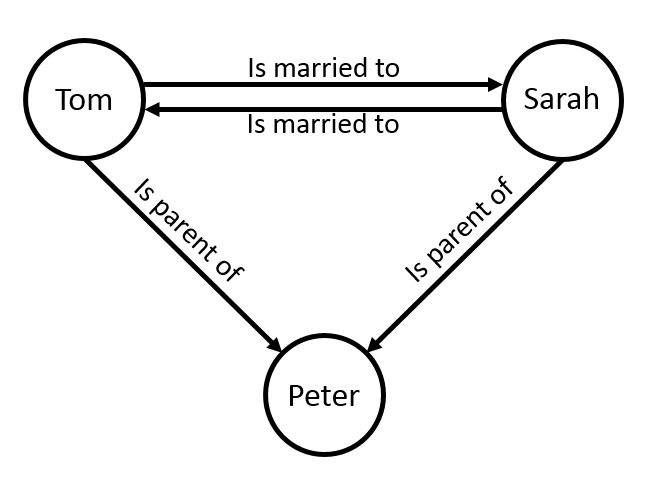
\includegraphics[width=.5\textwidth]{img/graph_example.PNG}
    \caption{A graph representing a small family. Tom, Sarah and Peter are entities and thus represented as nodes (circles). The two-way relationship between Tom and Sarah, their marriage, is depicted as two directed edges. Lastly, Tom and Sarah are the parents of Peter and thus both have the relationship "Is parent of" directed towards Peter.}
    \label{fig:graphdb:graph_example}
\end{figure}



\subsubsection{The property graph model}
The (labeled) property graph model is based on the theoretical graph from above \autocite{maheshlal2015}. It increases the overall information that a normal graph can store. Two such extensions, as the model name illustrates, are additional labels for each node and properties for nodes and edges. Figure \ref{fig:graphdb:property_graph_example} shows a labeled property graph.

\begin{figure}[ht]
    \centering
    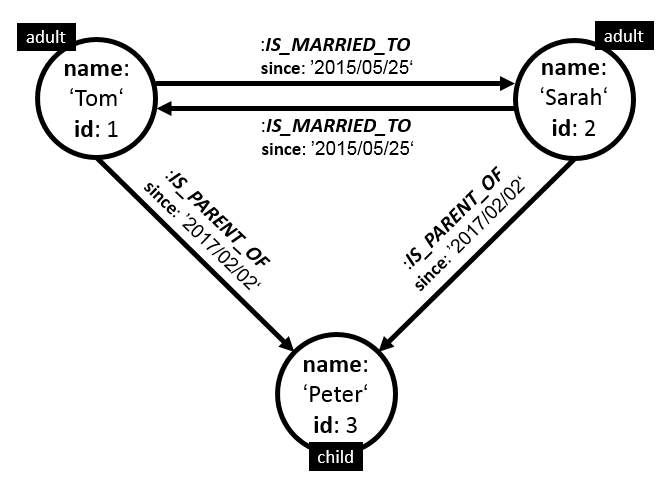
\includegraphics[width=.5\textwidth]{img/property_graph_example.PNG}
    \caption{A labeled property graph representing a small family \autocite{maheshlal2015, graphdb2015}. Compared to figure \ref{fig:graphdb:graph_example} additional information can been stored.}
    \label{fig:graphdb:property_graph_example}
\end{figure}

\scalebox{1}{\textbf{Concepts of the property graph}}

\textbf{Nodes:} Like a normal graph, the property graph represents entities as nodes. The nodes in figure \ref{fig:graphdb:property_graph_example} are the circles of Tom, Sarah and Peter. Each node can have any number of properties (e.g.: "name: ‘Tom’" and  "id: 1") and multiple labels (e.g. " adult") \autocite{neo4j:graphdb}.

\textbf{Labels:} Nodes are tagged with labels which describe the role of the node within the system \autocite{maheshlal2015}. In figure \ref{fig:graphdb:property_graph_example}, the white text on black rectangles, "adult" and "child", are labels. Labels can also add metadata (constraints and indices) to the node \autocite{maheshlal2015, neo4j:graphdb}.

\textbf{Properties:} Properties are attributes (key-value pairs) of nodes or relationships. They are used to sore further information about the entity or relationship \autocite{maheshlal2015}. Each bold and non-italic written word in figure \ref{fig:graphdb:property_graph_example} is a key of a key-value pair property (e.g. "name:", "id:", "since:"). The content that follows the colon (e.g. "Peter", "3", "2017/02/02") is the value.

\textbf{Relationships:} Again, relationship are depicted as directed edges (links) between nodes. Relationships must have a name as well as a start and end node \autocite{graphdb2015} . In figure \ref{fig:graphdb:property_graph_example}, \texttt{"IS\textunderscore PARENT\textunderscore OF"} and \texttt{"IS\textunderscore MARRIED\textunderscore TO"} (the italic and bold written words) are the names of relationships. The text below ("since: […]") is the property of the relationship. Arrows indicate the direction of the relationship.  In practice, the direction is ignored and navigation through each edge (relationship) is possible \autocite{maheshlal2015, neo4j:graphdb}. Generally, relationships store cost quantities according to the usage of the system (e.g. distance, ratings, etc.) \autocite{neo4j:graphdb}.

\subsubsection{Storage}
\blockquote{Storage deals with how the data is stored physically and how it is represented logically when retrieved}\autocite{maheshlal2015}

One of the main tasks of a graph database system is to traverse relationships. As mentioned earlier, storing and accessing the relationships in a graph database is crucial. They are stored explicit (per directed edge) instead of being inferred from stored attributes (like primary/foreign keys in a relational model) \autocite{maheshlal2015} . Thus, any kind of storage system needs to be able handle the relationships explicitly. Graph databases can either use native graph storage, systems that are built for storing and accessing graphs, or non-native graph storage, systems that store adequately transformed graph data in relational or non-graph \gls{nosql} databases \autocite{graphdb2015}.

\scalebox{1}{\textbf{Non-native graph storage}}

Non-native graph storage transforms the data from the graph model (e.g. property graph) into relational or other non-graph \gls{nosql} database models (document-oriented, etc.). When accessing the data, the responsible system must rebuild (infer) the relationships at runtime. This is mostly done by a query engine which is responsible for executing incoming queries and thus fetching or changing the data (\gls{crud} methods) \autocite{maheshlal2015} . In the case of a \gls{rdbms}, the query engine would first make the relationships explicit by inferring them through utilizing foreign keys and join-statements before returning or processing the data. This preprocessing results in more costly operations and inefficient traversing of relationships \autocite{maheshlal2015}. Non-native graph storage exists because it allows the use of well known, mature and well documented databases like MySQL \autocite{graphdb2015}.

\scalebox{1}{\textbf{Native graph storage}}

The key aspect of native graph storage is that it does not rely on actual indexes. The relationships between nodes within the graph are “natural adjacency”\autocite{graphdb2015}  indices. Thus, the nodes are stored in such a way that they are physically linked to each other on the disk. This is called “index-free adjacency”\autocite{graphdb2015}, which is in practice done by pointers. Accordingly, searching for a specific information in a native graph storage is implemented by traversing through pointers. This causes queries on native storage to be highly efficient compared to non-native storage which uses join-statements and index lookups \autocite{graphdb2015} .

\subsection{Advantages of Graph Databases}
Graph databases offer substantial advantages when working with connected data \autocite{maheshlal2015}. Its performance, flexibility and agility are the key differences to other databases \autocite{graphdb2015}. The following section will take a closer look at these three advantages. More details and references to actual research data on these advantages can be found in the section Comparison: Graph Databases and Relational Databases (\ref{graphdb:comparison}).

\subsubsection{Performance}
A graph database has much higher query processing performance compared to relational and other \gls{nosql} databases. This advantage becomes more and more prevalent as the size/amount of stored data grows. In the relational world more data would mean a higher join-intensity and thus worse performance. Whereas in the graph database world the performance remains to be almost constant even for an exponential increase of size. This is the cases because queries are being restricted to parts of the graph (e.g. a subgraph) which contains the information of interest.  Therefore, querying only needs time proportional to size of the subgraph and not to the size of the whole graph \autocite{maheshlal2015, graphdb2015}.

\subsubsection{Flexibility}
The flexibility of a graph databases must be understood in the context of the graph database model. The model is flexible and so are graph databases. Furthermore, this flexibility is most apparent for an actual operational graph database in production environments.

The paradigm of fitting data to predefined data models, as in \gls{sql}, is neither efficient nor desired by developers. Instead fitting an easily extensible and changeable data model to newly emerging data is more appropriate for fields of graph database applications (See more in the section "Fields of Application”, \ref{graphdb:FoA}). Thereby the process of designing a complex and mostly final data model at the start of the database implementation, a point in time where it is impossible to predict all kinds of data that might be needed in the future, gets replaced by designing a basic data model with the expectation to change it in the future \autocite{maheshlal2015, graphdb2015}.

This process is natively supported by graph databases. All components of a graph model (e.g. for the property graph model: nodes, properties, labels and relationships) can be added to an existing model without invalidating queries already in use. This concept of graph databases also minimizes maintenance cost and risk because the need for migrations (e.g. the equivalent of schema migrations for a relational database) is reduced \autocite{maheshlal2015, graphdb2015}.

\subsubsection{Agility}
In today's agile software development world, where developers need to focus on a certain task for a short time before switching to a different task, software tools that fit this iterative approach are more favorable. Databases that offer data models which can grow with new data meet this requirement. Additionally, databases that offer data models which do represent the data closer to its actual format (e.g. not transferring it into tables) are also more favorable because they reduce the time between design and implementation which is appropriate for the short time a developer may have to implement a database. Lastly, modern test-driven development requires agile databases to be easily testable. \autocite{maheshlal2015, graphdb2015}.

A graph database is “schema-less” \autocite{maheshlal2015}. It does not transform data (e.g. normalization in the \gls{sql} world) but rather tries to represent the data as close to its actual format as possible. Furthermore, the \gls{api} and query language design of graph database increase testability \autocite{graphdb2015} . Finally, the flexibility of its data model enables the database to evolve with new data. As a result, a graph database has the characteristics to be agile software.

\subsection{Fields of Application} \label{graphdb:FoA}
When reading through use cases described by marketing teams of graph database management systems (for example: Neo4j \autocite{neo4j:why_graphdb, neo4j:use_cases}
), it may feel like any problem could be solved with a graph database. Solving any problem with a graph database may be possible but this fact alone is not a valid reason to do so.

Instead, cost efficiently, compliance with company polices, available developer skills and available time are the primary reasons to choose a graph database for a specific use case. Additionally, replacing existing well-working and established database management systems should have major and urgently needed advantages \autocite{graphdb2015}.

Graph databases can create these advantages for use cases which handle connected data. Below are some short examples of large companies that use graph databases. Subsequently, the top five use cases from the perspective of the graph database management system Neo4j are explained.

\subsubsection{Enterprise Use Case Examples}
\textbf{Social Networks:} Twitter, Facebook and LinkedIn use graph databases to manage user information and feed of users. This contains information like updates from friends, news and potential posts of relevance or interest (e.g. Jobs for LinkedIn users) \autocite{maheshlal2015}.

\textbf{Routing:} Prominent navigation services like Google Maps, TomTom and Sygic utilize graph databases for map navigation \autocite{maheshlal2015}.

\textbf{Search:} Google (Google Knowledge Graph) and Facebook (Facebook Social Graph) are also using graph databases for storing the connection of content for search functionalities \autocite{maheshlal2015}.

\textbf{Recommendation:} Walmart and eBay are both using graph databases and value their performance for real-time product recommendations \autocite{neo4j:use_cases}.

\subsubsection{Neo4j Use Cases}
\scalebox{1}{\textbf{Fraud Detection}}

Graph databases are well fit for fraud detection because good detection mechanisms need to analyze the relationships between data. In detail, if the relationships between certain data objects is conspicuously high, the risk of fraud is very high.  As an example, take an E-commerce system. A normal user would use one or two credit cards to buy products. A fraudster would use a lot of different credit cards which are most likely stolen. This relationship density between users, credit cards and purchased products is modeled by a graph database and is therefore easily measurable and observable \autocite{neo4j:use_cases}.

As mentioned before, graph databases are built for storing and rapidly traversing relationships, thereby supporting advanced detection mechanisms that need to perform relationship analysis between a lot of data.

\scalebox{1}{\textbf{Real-Time Recommendation Engines}}

A real-time recommendation engine can only be as effective as the database it is using because the engine needs information about the existence, quality and strength of data relationships. Information must either be computed from the database in a time-consuming manner or made available natively, as with graph databases \autocite{neo4j:use_cases}. Graph databases model this information without any additional computation. Existence is modeled by edges (relationships), quality and strength by key-value pairs (properties) of edges.

In addition, the need to easily add and combine data (e.g. user behavior, demographics and their purchase history) and then analyze this new dataset in real time for possible recommendations is crucial for such an engine \autocite{neo4j:use_cases}. A graph database supports simple addition and combination with its already mentioned flexibility. Furthermore, the performance advantage of graph databases in this context is again very favorable when analyzing this new dataset.

\scalebox{1}{\textbf{Master Data Management}}

In a company, master data is data such as users, customers, products, accounts, partners, sites and business units. Identifying, cleaning, storing and governing this data is called \acrfull{mdm}. Best practice for \gls{mdm} is to create one master data store which contains the data of the entire company. As a result, any business application that might create or use this data only uses only the same storage system. Hence, the master data store is one storage system for a lot of different applications which still needs to fully function in real time and might need to adapt to new business requirements. Thus, it must provide a purpose-built, dynamic and sometimes unconventional data model \autocite{neo4j:use_cases}. These requirements are perfectly matched by the flexibility and agility of a graph database.

\scalebox{1}{\textbf{Network and Information Technology Operations}}

The structural representation of an \gls{it} infrastructure network is a graph. Consequently, it should not be a surprise that a graph database is a good solution to model, store and serve requests for an \gls{it} infrastructure environment. Information in an \gls{it} infrastructure environment are for example device configurations, infrastructure interdependencies, any kind of event (log files, error messages, etc.) and administrative details. Systems that use such information can, in the event of a failure, inform the right administrator about what went wrong where and when in real time \autocite{neo4j:use_cases}.

A graph database is not only able to model the network in its native representation but is also able to add all this information to its storage with ease. Network administrators are nodes with connection to their devices and field of responsibility (subgraphs). Configurations are properties of device nodes. Any interdependencies are represented by relationships. Lastly, events are nodes linked to the device that created it. This requirement for a native data model and sufficient performance is fulfilled by a graph database.

\scalebox{1}{\textbf{Identity and Access Management}}

The process of deciding which identity can access which resource is called \acrfull{iam}. This decision process also needs to utilize information about identities (e.g.  administrators, users), resources (e.g.  files, devices) and rules (e.g. “user X can access file Y”) that must be stored somewhere. Conventional storage options, like directory services or application specific solutions, tend to be unsuitable because they cannot manage the required complex interconnection structures of big organizations or are too slow for bigger datasets \autocite{neo4j:use_cases}.  Whereas a graph database is a valid solution because its agility allows the developer to easily model the complex structures and its performance does not slow down for bigger datasets.


\subsection{Comparison: Graph Databases and Relational Databases} \label{graphdb:comparison}
The comparison between Graph Databases and Relational Databases is a known field, a lot of literature exists on this topic already. Throughout the comparisons, the two methods are always assessed under the same aspects: performance, flexibility, security and maturity. \\
For those comparison points it makes sense to focus on specific implementations of the technologies, hence in this section Neo4j will be chosen as a concrete precedent for Graph Databases, whereas MySQL will be the example implementation for Relational Databases. \\
It is important to note that literature comparing the two is already rather old and there are no comparisons done on newer versions. There is no new version of mySQL, but two new releases for Neo4j. Those have included a new query engine and performance optimizations. It is hence expected that if such a comparison were to be done again today, the performance results of Neo4j would improve.

\subsubsection{Performance} \label{sec:graphdb:performance}
Detailed surveys on performance of both technologies already exist in literature, for example from Vicknair et al. \autocite{Vicknair2010}. In this specific instance, MySQL version 5.1.42 and Neo4j-b11 were compared.
The queries chosen for the experiments were similar to types that are used in real world provenance systems. Typically in this scenario, for one node one traverses the graph to find its origin. Another use case in this context is, if a data object or node is deemed incorrect, this information needs to be propagated to all its descendants/child nodes \autocite{Vicknair2010}.\\
Further on, the queries were partitioned into structural queries referencing the graph but not the payload itself, and data queries using the actual payload data. It is important to note that the payload data in this case was integer payload data, as different types are handled separately depending on the framework.\\
In the traversal queries, Neo4j clearly outperformed MySQL, sometimes even being faster by the factor of 10. Though that was expected, as Relational Databases are not designed for traversals. MySQL for this part of experiment falls back to a standard Breadth First Search, which is not optimal for this scenario. Neo4j on the other hand has a built in framework for traversals, making it superior in terms of performance for the traversal queries \autocite{Vicknair2010}. \\
Contrary to that, in the data queries MySQL turned out to be more efficient. This result was partly due to the fact that Neo4j uses Lucene for querying, which treats all payload as text, even though in this scenario the payload is of type integer. But also when the payload changes to text, MySQL had better performance in the experiments \autocite{Vicknair2010}. Lucene has since been dropped and replaced with Cypher in Neo4j version 3.\\
The researchers also took into account a special case for the experiments, trying the data queries with payload that is closer to actual real world data - text with spaces in between the words. Surprisingly, at a large enough scale Nao4j outperformed MySQL by a large amount for those queries.

\subsubsection{Flexibility}
The flexibility aspect compares both database technologies in their behaviour when taken out of the environment that they were created for \autocite{Vicknair2010}. \\
For Relational Databases an uncommon environment would for example be ad-hoc data schemes that change with time, whereas for Graph Databases a less typical dataset would be one without many connections between the individual nodes  \autocite{GarimaAnalysis}.
MySQL is optimized for a large-scale multi-user environment, hence trying to use it for smaller applications comes with a large overhead of functionality that has to be implemented with it but that may not even be needed for this specific application.
Neo4j is typically targeted towards more lightweight applications, but manages to scale really well, having a scalable architecture that also accounts for speed \autocite{neo4jweb}. Its easily mutable schema makes it more flexible with data types that are rather untypical for Graph Databases.

\subsubsection{Security}
Neo4j does not have built in mechanisms for managing security restrictions and multiple users in their community edition \autocite{GarimaAnalysis}, but the fee-based enterprise edition provides such functionality. MySQL on the other hand natively supports multiple users as well as access control lists. \autocite{mysqlsecurity}

\subsubsection{Maturity}
For the comparison under the aspect of maturity it makes sense to talk about database implementations in general. Maturity refers both to how old a particular system is and to how thoroughly tested it is \autocite{Vicknair2010}.
Since all Relational databases - including MySQL - use the same query language \gls{sql}, support is equal over all implementations and support for one implementation is applicable to all others \autocite{GarimaAnalysis}.
Neo4js version 1.1 was released in February 2010. While Neo4j is a for-profit framework and has decent support from its parent company, this does not apply to all graph database implementations \autocite{Vicknair2010}. Furthermore, the query languages differ from implementation to implementation, separating them in that aspect and making support for one implementation not applicable to another one.

\section{Implementing a Graph Database Model} \label{graphdb:section3}
This section shall outline the general approach, how to convert an existing relational database model into a property graph model.
In the second part an introduction to Neo4j, the implementation of a database model in Python and basic querying in an application and with Neo4js own query language \glqq Cypher\grqq{} will follow.

\subsection{Converting a Relational Database Model}
There are a couple of guides available describing how to build a database model for Neo4j. Since the database itself is schema-less, multiple schemas can be used and implemented at the same time.
Nevertheless an application needs a model of the data.
Neo4j states in \autocite{neo4j:rel_to_graph} that it is possible to transfer almost all existing relational models into a graph model.
The general approach has been described in \autocite{dzone:rel_to_graph}.
The first step in this conversion is to consider the names of all Non-JOIN-Tables as labels.
Foreign keys will become relations.
JOIN-Tables will be converted into relations as well with additional properties added to the relation \autocite{neo4j:graph_vs_rdbms}.
The rows will be converted into nodes connected by edges based on the formerly converted relations. Attributes not covered in the previous steps will become properties of a node.

\subsection{Implementing a Sample Project with Neo4j}
In this section the modeling and setup with Neo4j will be lined out and a sample project be described utilizing available Python-Libraries to implement a sample project.
There are two different available versions of Neo4j.
First of all there is the Open Source community edition which is published under the GPL.
Additionally Neo4j Inc sells licenses for an enterprise edition \autocite{neo4j:editions} including support and several additional features, such as replication, multiple users, several query performance optimizations and no limitation for the number of nodes in the database (the community version is limited at 34 Billion nodes).
The following examples have been implemented and tested with the community edition.

\subsubsection{Setting up Neo4j}
Neo4j is available for Windows, Linux and Mac and can be installed via the provided packages. While there is a minimum requirement of 2GB of RAM, Neo4j recommends 16GB or more \autocite[Chapter~2.1]{neo4j:op_manual}.
Since Neo4j is implemented in Java, starting it can be done by invoking it with a Java runtime of choice installed. The default configuration does not need to be modified to get started.

\paragraph{High availability} \label{par:graphdb:ha} The community edition of Neo4j does not allow to set up a cluster of multiple Neo4j instances.
This feature is reserved for the enterprise version.
The setup of a causally consistent cluster is explained in the documentation \autocite[Chapter~5.1]{neo4j:op_manual}.
The reference architecture as shown in \autoref{fig:graphdb:causal_cluster} recommends an odd number of at least three \glqq Core Servers\grqq{} connected into a RAFT-Cluster handling mostly write requests.
They ensure consistency of the data.
Connected to this core cluster may be an arbitrary number of \glqq Read Servers\grqq.
They only handle the -- sometimes resource costly -- read requests but are not relevant to the clusters integrity.
Information from Core Servers is replicated asynchronously to the read replicas.
\begin{figure}[ht]
    \centering
    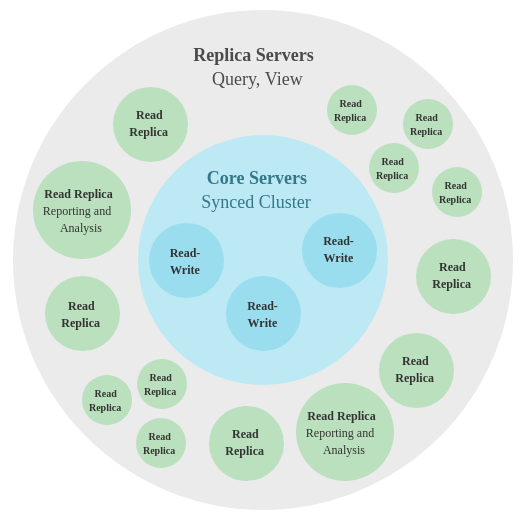
\includegraphics[width=.5\textwidth]{img/causal_clustering.png}
    \caption{Neo4j causal Cluster Architecture \autocite[Chapter~5.1]{neo4j:op_manual}}
    \label{fig:graphdb:causal_cluster}
\end{figure}

\paragraph{Classification of Neo4j within the CAP Theorem} For this kind of classification it is again necessary to differentiate between the community and the enterprise edition.
Since it is not possible to set up a Neo4j-Cluster with the community edition it can not be considered a distributed system.
Therefore the CAP-Theorem is not applicable \autocite{dzone:understanding_cap}.

As mentioned in \autoref{par:graphdb:ha} the enterprise edition can be set up as a causal cluster.
Causal consistency though does not fulfill the criteria Brewer put out for consistency \autocite{DBLP:journals/corr/Kleppmann15} so it can not be considered as \glqq C\grqq{} under the CAP Theorem.
It is important to note that a causal cluster is still ACID compliant.
Due to the nature of the core servers using a consensus-based protocol (RAFT) availability in case of a network partition only applies to the majority of the cluster \autocite{infoq:neo4j}.
This does make them partition tolerant though, fulfilling all criteria for \glqq P\grqq.

According to Michael Hunger, one of the Neo4j developers, the causal cluster architecture can be considered as a \glqq CP\grqq{} system \autocite{infoq:neo4j}.
Considering the the concerns lined out by Martin Kleppmann in his blog post \autocite{kleppmann:caprant} Neo4j should be considered as \glqq P\grqq{} -- if no alternative to CAP is considered as proposed by him \autocite{DBLP:journals/corr/Kleppmann15}.


\subsubsection{Modeling the graph database}
The sample project maps the relations within users in a social network.
\autoref{fig:graphdb:graphmodel} outlines a data model with circles representing nodes. They are connected by edges showing their relationships.
For this example labels are represented as colours.
In this sample model there may be an arbitrary number of persons (orange), who may be friends with other persons.
Additionally, they can share interests (green) and may be a member of a group (purple).
Furthermore they can state from which country (yellow) they are from.

\begin{figure}[H]
    \centering
    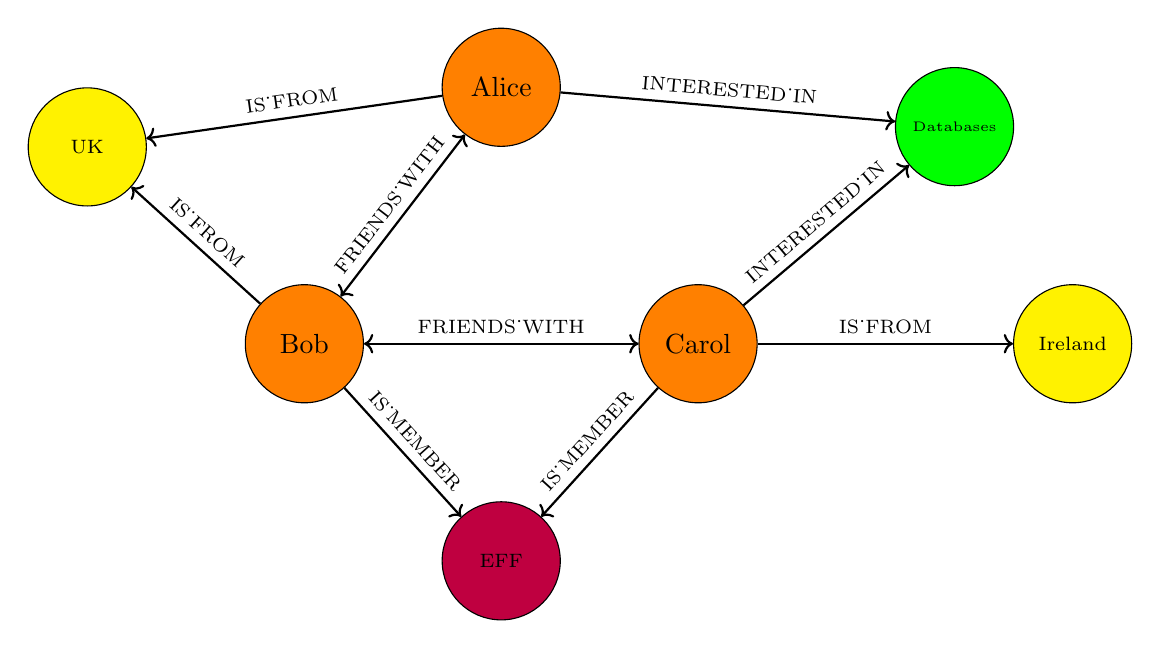
\begin{tikzpicture}
        \node[draw, circle, fill=orange, minimum height=1.5cm, minimum width=1.5cm] (alice) {Alice};
        \node[draw, circle, fill=orange, minimum height=1.5cm, minimum width=1.5cm] (bob)  at ([xshift=-2.5cm, yshift=-2.5cm]alice.south) {Bob};
        \node[draw, circle, fill=orange, minimum height=1.5cm, minimum width=1.5cm] (carol)  at ([xshift=2.5cm, yshift=-2.5cm]alice.south) {Carol};

        \node[draw, circle, fill=green, minimum height=1.5cm, minimum width=1.5cm] (db) at ([xshift=5cm, yshift=-0.5cm]alice.east) {\tiny Databases};

        \node[draw, circle, fill=purple, minimum height=1.5cm, minimum width=1.5cm, align=center] (eff) at ([xshift=2.5cm, yshift=-2cm]bob.south) {\scriptsize EFF};

        \node[draw, circle, fill=yellow, minimum height=1.5cm, minimum width=1.5cm] (uk) at ([xshift=-2cm, yshift=2.5cm]bob.west) {\scriptsize UK};
        \node[draw, circle, fill=yellow, minimum height=1.5cm, minimum width=1.5cm] (ire) at ([xshift=4cm]carol.east) {\scriptsize Ireland};



        \draw [<->, thick] (alice) -- (bob) node[midway,sloped, above] {{\scriptsize FRIENDS\char`_WITH}};

        \draw [<->, thick] (bob) -- (carol) node[midway,sloped, above] {\scriptsize FRIENDS\char`_WITH};

        \draw [->, thick] (alice) -- (db) node[midway,sloped, above] {\scriptsize INTERESTED\char`_IN};
        \draw [->, thick] (carol) -- (db) node[midway,sloped, above] {\scriptsize INTERESTED\char`_IN};

        \draw [->, thick] (bob) -- (eff) node[midway,sloped, above] {\scriptsize IS\char`_MEMBER};
        \draw [->, thick] (carol) -- (eff) node[midway,sloped, above] {\scriptsize IS\char`_MEMBER};

        \draw [->, thick] (alice) -- (uk) node[midway,sloped, above] {{\scriptsize IS\char`_FROM}};
        \draw [->, thick] (carol) -- (ire) node[midway,sloped, above] {{\scriptsize IS\char`_FROM}};
        \draw [->, thick] (bob) -- (uk) node[midway,sloped, above] {{\scriptsize IS\char`_FROM}};

    \end{tikzpicture}
    \caption{Sample database schema}
    \label{fig:graphdb:graphmodel}
\end{figure}

\subsubsection{Implementation in Python}
While it is possible to manage the database utilizing the \gls{crud}-functionality from Neo4js own query language Cypher (see \ref{sec:graphdb:cypher}) this is not really suitable for an application.
Developers familiar with \glspl{orm} such as Hibernate for Java or SQLAlchemy for Python would prefer to define the different nodes and relations in classes providing the database elements as objects and abstracting actual \gls{sql}-Queries.

For Python there exists a community driven project called neomodel \autocite{github:neomodel} aiming to provide an \gls{ogm} for Python projects. Neomodel is published under the MIT License.

\begin{listing}[ht]
    \begin{minted}{python}
    class Partnership(StructuredRel):
        since = DateTimeProperty(
            default=lambda: datetime.now(pytz.utc)
        )

    class Country(StructuredNode):
        name = StringProperty(unique_index=True, required=True)

    class Interest(StructuredNode):
        name = StringProperty(unique_index=True, required=True)

    class Group(StructuredNode):
        name = StringProperty(unique_index=True, required=True)

    class Person(StructuredNode):
        uid = UniqueIdProperty()
        name = StringProperty(unique_index=True)
        age = IntegerProperty(index=True, default=0)

        # traverse outgoing relations
        country = RelationshipTo(Country, 'IS_FROM')
        interests = RelationshipTo(Interest, 'IS_INTERESTED_IN')
        groups = RelationshipTo('Group', 'IS_MEMBER')
        friends = Relationship('Person', 'FRIENDS_WITH', model=Partnership)
    \end{minted}
    \caption{Example graph database model with neomodel}
    \label{lst:graphdb:neomodel}
\end{listing}

The implementation of the graph model mentioned in \autoref{fig:graphdb:graphmodel} in Python has been realized in \autoref{lst:graphdb:neomodel} following the neomodel documentation \autocite{neomodel:rtd}. With this model it is possible to create new nodes in the database by instantiating a new object of the given classes as in \autoref{lst:graphdb:createPerson}.
\begin{listing}[H]
\begin{minted}{python}
lmeitner = Person(name='Lise Meitner', age=89)
lmeitner.save()
\end{minted}
\caption{Creating a new person node in the database}
\label{lst:graphdb:createPerson}
\end{listing}

To connect two nodes it is necessary to get both objects and to invoke the \texttt{connect()} method as seen in \autoref{lst:graphdb:connectNodes} on one of them.
The \texttt{get\char`_or\char`_create} method simplifies creation of nodes with no additional properties since it either returns an already existing node or creates it.
\begin{listing}[H]
\begin{minted}{python}
country = Country.get_or_create({'name': 'Austria'})
lmeitner.country.connect(country[0])
\end{minted}
\caption{Connecting a person and a country node}
\label{lst:graphdb:connectNodes}
\end{listing}

Retrieving one or more existing nodes can be done by filtering as shown in \autoref{lst:graphdb:queryPerson}.
\begin{listing}[H]
\begin{minted}{python}
curie = Person.nodes.filter(name='Marie Curie')
\end{minted}
\caption{Querying for a person node by the name attribute}
\label{lst:graphdb:queryPerson}
\end{listing}

\subsubsection{Queries using Cypher}
\label{sec:graphdb:cypher}
Neo4j provides its own query language Cypher. It is developed with an open source specification called openCypher \autocite{openCypher}.
Thus it should be possible to use the same query language for graph processing in other databases -- such as SAP HANA or Redis.
Its syntax is oriented on \gls{sql} statements though there are quite some differences to better match with a graph model.
Neo4j has an extensive introduction how to use Cypher \autocite{neo4j:cypher_introduction}.
Therefore only a short introduction should be given here.

Cypher uses two basic patterns.
First of all there are nodes, denoted by enclosing parentheses.
The second pattern is used for relationships.
They are expressed by two dashes and may have a direction utilizing the greater-than/less-than signs.
Furthermore, the type of a relationship may be specified in brackets between the two dashes.

A few examples will make it easier to understand how these patterns can be used.

The simplest query would be to get all nodes and all relations between them without regard to their labels.
This can be achieved by calling \mint{SQL}|MATCH (n) RETURN n|
It is important to note that Cypher uses \texttt{MATCH} as a keyword similar to \gls{sql}'s \texttt{SELECT}.
Contrary to \gls{sql} it is necessary in Cypher to \texttt{RETURN} the previously matched nodes to obtain them in the result.
It is possible to declare the label of a node by calling \mint{SQL}|MATCH (p:Person) RETURN p|
This would reduce the output to all persons and the relations between them.

As mentioned before Cypher supports a pattern for relations.
To include them in a query -- e.g. for all Persons who have one or more friends the query would look like \mint{SQL}|MATCH (a:Person) -[:FRIENDS_WITH]- (b:Person) RETURN a, b|
The relationship type in the brackets may be ommited to get all types of relations between these nodes.

Similar to SQL, Cypher also supports a \texttt{WHERE} statement.
To query for a specific Person where the attribute \texttt{name} equals \glqq Otto Hahn\grqq{} and all nodes connected to this person the Cypher query would look like this \mint{SQL}|MATCH (p:Person)-[r]-(n) WHERE p.name = 'Otto Hahn' RETURN p, r, n|

Of course Cypher offers a complete keyword set for all types of \gls{crud} operations. Interested readers should follow the introduction by Neo4j \autocite{neo4j:cypher_introduction}.

\subsection{Conclusion}
Getting started with Neo4j is relatively simple.
There is plenty of documentation available helping to implement a database model and an application based on it.
Especially the \gls{ogm} Projects for Python are pretty advanced and suitable for production usage.
Users familiar with \gls{sql} will find Cypher not that difficult to get used to.

There are two major downsides to Neo4j. The first one is the memory footprint.
A newly set up instance already consumes more than 600MB of RAM -- in comparison, a PostgreSQL instance storing a couple hundred MB of data still consumes less than half of that.
The second downside is, that many features -- especially regarding maintenance and clustering -- are preserved for the enterprise edition and not available in the open source community edition. This makes it difficult if not impossible to use the community edition in a production environment.

\section{Reflection} \label{graphdb:section4}
\subsection{Alternative Graph Databases}
\subsubsection{OrientDB}
OrientDB is one of the biggest competitors to Neo4j, developed by Callidus Software Inc. (owned by SAP) and published under Apache-2 License \autocite{orientdb:vs_neo4j}.
Like Neo4j it is implemented in Java.
OrientDB is a multi model graph database, just as Neo4j, but also a document oriented database allowing relations between documents \autocite{orientdb:why}.
As a query language OrientDB uses \gls{sql} with a custom dialect to include features for traversals \autocite{orientdb:vs_neo4j}.
In comparison to Neo4j they claim to be a lot faster \autocite{orientdb:vs_neo4j}.
This claim is based on a paper \autocite{cloudcom:2012}, which has been released in 2012.
As mentioned in \autoref{sec:graphdb:performance} Neo4j has reimplemented their query engine since then.


A major selling point is the possibility to set up a highly-available (multi-master) cluster of multiple nodes with the Open Source community version \autocite{orientdb:cluster, orientdb:support}.

\subsection{Conclusion}
Even though there is extensive literature on the topic of Graph Databases, our group was overall dissatisfied with the scientific resources we found. Most publications were written by the same few people, not providing a distinct enough reflection on the topic. Furthermore, while there were many publications around 2010 on this topic, literature did not provide updates or added benchmarks of e.g. comparisons with other database systems. We aim to close that gap with an updated summary on today's Graph Database theory and Neo4j. \\
In this chapter, we first gave an introduction into Graph Databases, providing an overview of its history. Next, the basic underlying theory was explained and assessed critically. A report on the implementation with Neo4j was given, stating its distinct characteristics and concluding its value as a Graph Database implementation.

To conclude, we would also like to share our personal experience of working with Neo4j and Graph Databases in general. Overall, we feel that with the concept of Graphs as a database model one can easier map real life datastructures than with just a relational structure. While the underlying theory is rather complex, we felt that there were sufficient resources to give a simple introduction into the topic. The implementation was enjoyable, as the documentation for Neo4j was easily understandable and it did not take long until the basic setup was complete. We especially enjoyed using community driven libraries; when issues arose we were given an answer and help immediately, making our experience overall very pleasant.

Future work to extend this paper could include assessing the enterprise edition. We were unable to compare the community edition to the enterprise edition due to stellar pricing. The fee-based version allows for clustering which would have been interesting to take into account for our implementation. In addition, a deeper evaluation of alternatives like OrientDB could be valuable, especially since OrientDB is an open source project and provides clustering functionality in its community version. Lastly, Hypergraph and Triplet propose interesting approaches to graph modeling and an assessment of the differences and strengths would be valuable for the current literature landscape.



\printbibliography

\appendix
%!TEX root = ../main.tex

\chapter{Cassandra query example}\label{appendix:cassandra:queryExample}
\begin{verbatim}
Create database, table, insert and select data

CREATE KEYSPACE people
    WITH REPLICATION =
      { 'class' : 'SimpleStrategy', 'replication_factor' : 3 };
USE people;

CREATE COLUMNFAMILY users (
    username varchar PRIMARY KEY,
    name varchar,
    lastname varchar,
    email varchar,
    age int
);

INSERT INTO users (username, name, lastname, email)
    VALUES ('john', 'John', 'Smith', 'john@gmail.com');
INSERT INTO users (username, name, lastname, age)
    VALUES ('jack', 'Jack', 'Sparrow', 33);
INSERT INTO users (username, name, lastname, email, age)
    VALUES ('kate', 'Kate', 'Austen', null, 25);

SELECT * FROM users;

 username | age  | email          | lastname | name
----------+------+----------------+----------+------
     kate |   25 |           null |   Austen | Kate
     john | null | john@gmail.com |    Smith | John
     jack |   33 |           null |  Sparrow | Jack

$ nodetool flush

$ sstabletump /var/lib/cassandra/data/people/*/mc-1-big-Data.db
[
  {
    "partition" : {
      "key" : [ "kate" ],
      "position" : 0
    },
    "rows" : [
      {
        "type" : "row",
        "position" : 45,
        "liveness_info" : { "tstamp" : "2019-04-14T16:21:05.014317Z" },
        "cells" : [
          { "name" : "age", "value" : 25 },
          {
            "name" : "email",
            "deletion_info" :
              { "local_delete_time" : "2019-04-14T16:21:05Z" }
          },
          { "name" : "lastname", "value" : "Austen" },
          { "name" : "name", "value" : "Kate" }
        ]
      }
    ]
  },
  {
    "partition" : {
      "key" : [ "john" ],
      "position" : 46
    },
    "rows" : [
      {
        "type" : "row",
        "position" : 98,
        "liveness_info" : { "tstamp" : "2019-04-14T16:21:04.982207Z" },
        "cells" : [
          { "name" : "email", "value" : "john@gmail.com" },
          { "name" : "lastname", "value" : "Smith" },
          { "name" : "name", "value" : "John" }
        ]
      }
    ]
  },
  {
    "partition" : {
      "key" : [ "jack" ],
      "position" : 99
    },
    "rows" : [
      {
        "type" : "row",
        "position" : 144,
        "liveness_info" : { "tstamp" : "2019-04-14T16:21:05.002672Z" },
        "cells" : [
          { "name" : "age", "value" : 33 },
          { "name" : "lastname", "value" : "Sparrow" },
          { "name" : "name", "value" : "Jack" }
        ]
      }
    ]
  }
]
\end{verbatim}



\end{document}
